\documentclass[a4paper,11pt]{article}
\usepackage[lmargin=1.5cm,rmargin=1.5cm,bmargin=1.5cm]{geometry}
\usepackage[UKenglish]{babel}
\usepackage{graphicx}
\usepackage{courier}
\usepackage{color}
\usepackage{array}
\usepackage{pstricks}
\usepackage{parskip}
\usepackage[bottom]{footmisc}
\usepackage{fancyhdr}
\usepackage[none]{hyphenat}
% the hyperref package must always be the last package to be included
\usepackage[pdftex,
            pdfusetitle,
            pdfsubject={User's Manual for dastaZ80 homebrew computer},
            pdfkeywords={Z80, homebrew computer, Operating System, OS}
        ]{hyperref}

\hypersetup{
    colorlinks = true,
    linkcolor = blue,
    anchorcolor = blue,
    citecolor = blue,
    filecolor = blue,
    urlcolor = blue
}

\setlength\parindent{0pt}

\begin{document}
    \pagestyle{empty}
    % ==========================================================================
    % Cover page
    % ==========================================================================
    \begin{pspicture}(8.5,11)
        \rput[b](3.5,8){
            \parbox{10in}{
                \begin{flushright}
                    \Huge\bfseries\sffamily dastaZ80 Mark III\\ User's Manual
                \end{flushright}
            }
        }
        \uput[0](0,0){\color{blue}\rule{10in}{0.5ex}}
    \end{pspicture}
    \title{dastaZ80 User's Manual}
    \author{David Asta}
    \date{7 September 2022}

    \pagebreak
    % ==========================================================================
    % Header & Footer
    % ==========================================================================
    \pagestyle{fancy}
    \fancyhf{}
    \fancyhead[R]{dastaZ80 Mark III User's Manual}
    
    \begingroup
        \let\clearpage\relax
        % ==========================================================================
\section*{Disclaimer}
% ==========================================================================
The products described in this manual are intended for educational purposes,
and should not be used for controlling any machinery, critical component in
life support devices or any system in which failure could result in personal
injury if any of the described here products fail.

These products are subject to continuous development and improvement. All
information of a technical nature and particulars of the products and its
use are given by the author in good faith. However, it is acknowledged that
there may be errors or omissions in this manual. Therefore, the author
cannot accept any liability for any loss or damage arising from the use of
any information or particulars in this manual.

% ==========================================================================
\section*{Licenses}
% ==========================================================================
\small
\textbf{Hardware} is licensed under the \textbf{Creative Commons
Attribution-ShareAlike 4.0 International License}

\hspace{1cm}http://creativecommons.org/licenses/by-sa/4.0/

\textbf{Software} is licensed under \textbf{The MIT License}

\hspace{1cm}https://opensource.org/licenses/MIT

\textbf{Documentation} is licensed under the \textbf{Creative Commons
Attribution-ShareAlike 4.0 International License}

\hspace{1cm}http://creativecommons.org/licenses/by-sa/4.0/

\normalsize

\hrulefill
        
        \textcopyright 2023 David Asta
    \endgroup

    \pagebreak
    % ==========================================================================
    \section*{Document Conventions}
    % ==========================================================================
    The following conventions are used in this manual:

    \begin{center}
        \begin{tabular}{c m{14cm}}
            \hline
            MUST & MUST denotes that the definition is and absolute
            requirement.\\
            \hline
            SHOULD & SHOULD denotes that it is recommended, but that there may
            exist valid reasons to ignore it.\\
            \hline
            \textbf{DEVICE} & Device names are displayed in bold all upper case 
            letters, and refer to hardware devices.\\
            \hline
            \textbf{command} & Operating System command keywords are displayed 
            in bold all lower case letters.\\
            \hline
            \textit{$<$text$>$} & Angle brackets enclose variable information 
            that you MUST supply. In place of \textit{$<$text$>$}, substitute 
            the value desired. Do not enter the angle brackets when entering the
            value.\\
            \hline
            \textit{$[$text$]$} & Square brackets enclose variable information
            that you COULD supply. They are optional. In place of $[$text$]$,
            substitute the value desired. Do not enter the square brackets when
            entering the value.\\
            \hline
            \texttt{Courier} & Text appearing in the \texttt{Courier} font 
            represents information that you type in via the keyboard.\\
            \hline
            0x14B0 & Numbers prefixed by 0x indicate an Hexadecimal value.
            Unless specified, memory addresses are always expressed in
            Hexadecimal.\\
            \hline
            \textit{Return} & Refers to the key Return in the keyboard.\\
            \hline
        \end{tabular}
    \end{center}

    \hfill\break
    \hfill\break

    The SD card is referred as \textbf{DISK}.

    The Floppy Disk Drive is referred as \textbf{DISK} or as \textbf{FDD}.

    The 80 column text VGA output is referred as \textbf{CONSOLE} or as
    \textbf{High Resolution Display}.

    The 40 column graphics Composite Video output is referred as \textbf{Low
    Resolution Display}.
    
    The Operating System may be referred as DZOS, dzOS or simply OS.

    \textbf{MEMORY} refers to both \textbf{ROM} and \textbf{RAM}.

    Although the word \textbf{ROM} is used in this manual, the actual chip used
    in the dastaZ80 computer is of the type \textbf{EEPROM}.

    Memory used by the \textbf{Low Resolution Display} is referred as
    \textbf{VRAM} (Video RAM).

    \pagebreak
    % ==========================================================================
    \section*{Related Documentation}
    % ==========================================================================
    \begin{itemize}
        \item dastaZ80 User's Manual\cite{dastaz80userman}
        \item dastaZ80 Technical Reference Manual\cite{dastaz80techman}
        \item dzOS Github Repository\cite{dastaZ80github}
        \item Software for dzOS Github Repository\cite{dastaZ80githubsoft}
        \item Nascom 2 Microcomputer BASIC Programming Manuals\cite{nascombasic}
        \item Z80 Family CPU User Manual\cite{z80manual}
    \end{itemize}

    \pagebreak
    % ==========================================================================
    \tableofcontents
    % ==========================================================================

    \pagebreak
    % ==========================================================================
    % Header & Footer
    % ==========================================================================
    \pagestyle{fancy}
    \fancyhf{}
    \fancyhead[R]{dastaZ80 Mark III User's Manual}
    \fancyfoot[R]{\thepage}
    \setcounter{page}{1}
    % ==========================================================================
    \section{Introduction}
    % ==========================================================================
    The dastaZ80 is a homebrew computer designed and built following the style
    of the 8-bit computers of the 80s that I used on those days: Amstrad CPC,
    Commodore 64 and MSX. The name comes from “d”avid “asta” (my name) and 
    “Z80” (the CPU used).

    The idea behind the making of this computer came from an initial wish of
    writing an operating system (OS) for an 8-bit machine. Not comfortable with
    writing an OS for an already existing computer like an Amstrad CPC, C64,
    MSX, etc., due to the complexity of its hardware (or rather my lack of
    knowledge), I decided to built my own 8-bit computer from scratch, so that
    I could fully understand the hardware and also influence the design.

    The OS written by me for this computer is called \textit{DZOS}, from 
    dastaZ80 OS. Sometimes I spell it as \textit{dzOS}. Haven’t made my mind 
    yet.

    This manual describes the usage of DZOS running on the dastaZ80 computer.
    
    \pagebreak
    % ==========================================================================
    \section{dastaZ80 Overview}
    % ==========================================================================

    The dastaZ80 computer comes in two different formats:

    \begin{itemize}
        \item dastaZ80 (Original), in Acorn Archimedes A3010 case.
        \item dastaZ80DB (\textit{DB} stands for Desktop Box), in a desktop
            computer box.
    \end{itemize}

    Both are functionally the same, except the dastaZ80DB does not have a
    keyboard nor a Floppy Disk Drive, and is meant to be operated from an
    external video terminal (like DEC VT100) or a computer running a terminal
    program (like Minicom or PuTTY). More details about this configuration in
    the section \hyperref[sec:setting_system]{Setting up the system}.

    The dastaZ80 Original was the first version I made, and it is a stand-alone
    computer. Only things needed to use it are: the computer itself, a 5V/4A
    power supply, a monitor with VGA connector and optionally a monitor with 
    NTSC Composite video input and (also optionally) a pair of amplified
    speakers or a monitor with RCA stereo connectors.

    The dastaZ80DB requires the same, plus an external serial keyboard. Also,
    the VGA can be exchanged by a serial monitor.

    % ==========================================================================
    \subsection{dastaZ80 Original}
    % ==========================================================================

    \begin{itemize}
        \item ZiLOG Z80 microprocessor (CPU) running at 7.3728 MHz
        \item 64 KB RAM: 16 KB reserved for DZOS, 48 KB available
            for the user and programms.
        \item Storage devices: Micro SD Card\footnote{Formatted with FAT32 and
            containing Disk Image Files formatted with DZFS (dastaZ80 File
            System.)}, 3.5" DD/HD Floppy Disk Drive.
        \item Dual Video output: VGA 80 columns by 25 lines and 16 colours,
            Composite NTSC 15 colours.
        \item Stereo Sound: 3 channels (1 tone per channel), 7 octaves, 1 noise
            channel, envelope generator\footnote{Same chip (AY-3-8912 PSG) as
            used in numerous Arcade machines and in Amstrad CPC, Atari ST, MSX,
            ZX Spectrum and other home computers.}.
        \item Real-Time Clock: Date and Time backed up with button cell battery.
        \item Keyboard: Acorn Archimedes A3010 keyboard. 102 keys with 12 function
            keys, cursor keys and numeric pad.
        \item Case: Repurposed Acorn Archimedes A3010 case with keyboard.
        \item Expansion ports: GPIO and ROM Cartridges.
    \end{itemize}

    % ==========================================================================
    \subsection{dastaZ80DB}
    % ==========================================================================

    Same as above, with the only differences:

    \begin{itemize}
        \item No keyboard.
        \item No Floppy Disk Drive.
        \item Case: desktop box.
    \end{itemize}

    \pagebreak
    % ==========================================================================
\section{Setting up the system}
% ==========================================================================
\label{sec:setting_system}

% ==========================================================================
\subsection{dastaZ80 Original}
% ==========================================================================

You will only need:

\begin{itemize}
    \item The dastaZ80 computer.
    \item A 5 Volts (4 Amp) power supply with a female 2.1mm barrel-style DC
    connector (positive polarity).
    \item A Micro SD card.
    \item A monitor with VGA input.
    \item A LIR2032 Li-Ion Rechargeable 3.6V Battery Button Cell.
    \item Optionally:
    \begin{itemize}
        \item A monitor with NTSC Composite input.
        \item A 3.5mm jack to 3 RCA Audio/Video cable\footnote{This is the same
            cable used on the Raspberry Pi for Composite output}.
    \end{itemize}
\end{itemize}

% ==========================================================================
\subsection{dastaZ80DB}
% ==========================================================================

You will need:

\begin{itemize}
    \item The dastaZ80DB computer.
    \item Another computer, with serial port (either USB or RS-232).
    \begin{itemize}
        \item For USB, you will need a TTL-to-USB cable.
        \item For RS-232, you will need a TTL-to-RS-232 converter.
    \end{itemize}
    \item A 5 Volts (4 Amp) power supply with a female 2.1mm barrel-style DC
    connector (positive polarity).
    \item A Micro SD card.
    \item A LIR2032 Li-Ion Rechargeable 3.6V Battery Button Cell
    \item Optionally:
    \begin{itemize}
        \item A monitor with VGA input.
        \item A monitor with NTSC Composite input.
        \item A 3.5mm jack to 3 RCA Audio/Video cable\footnote{This is the same
            cable used on the Raspberry Pi for Composite output}.
    \end{itemize}
\end{itemize}

% ==========================================================================
\subsection{Lets put it together}
% ==========================================================================

\begin{enumerate}
    \item Insert the battery LIR2032 in the battery holder. Positive goes up.
    \item On a modern PC, format the SD card with FAT32.
    \item Create a file of 33 MB on the SD card.
    \begin{itemize}
        \item For example using Linux terminal: \texttt{fallocate -l \$((33*1024*1024)) dastaZ80.img}
    \end{itemize}
    \item Create a file named \textit{\_disks.cfg} in the root of the SD card,
    and add two lines to it:
    \begin{itemize}
        \item dastaZ80.img
        \item \#
    \end{itemize}
    \item Introduce the SD card in the SD card slot at the back of the
        computer case. This procedure MUST be performed with the computer
        switched off. For the dastaZ80DB, the SD card slot is at the front of
        the case.
    \item Connect the jack of the Audio/Video cable to the A/V connector at
        the back of the computer case. This procedure SHOULD be performed with
        the computer unplugged.
    \item Connect the female power supply connector to the male connector at
        the back of the case.
    \item For the dastaZ80 Original, connect the VGA cable from the monitor to
        the VGA connector at the back of the computer case. This procedure
        SHOULD be performed with the computer unplugged.
    \item For the dastaZ80DB, there are two options:
    \begin{itemize}
        \item Connect the TTL-to-USB cable to the 4 pins header labelled
            \textit{TTL I/O}, to have the input (keyboard) and output (screen)
            from/to another computer.
        \item Or, connect the TTL-to-USB cable to \textit{TTL I/O}, but also
            connect the VGA cable to the VGA connector, and set the switch in
            the front of the case (labelled \textit{TTL / VGA}) to the position
            \textit{VGA}. This way, the signal will be send to the VGA monitor
            and not to the other computer.
    \end{itemize}

\end{enumerate}

That’s really it. Switch the computer on, with the power switch, and you
should see text on your VGA monitor. DZOS is ready to use.

If your are using the dastaZ80DB with the TTL-to-USB cable for both input and
output, you need to open a terminal program in your other computer and set it up
to connect at 115,200bps 8N1 no hardware flow control. After flipping the
switch, you should see text on the terminal program.

Nevertheless, it's worth noting that by following this procedure the disk
image in the SD card will be empty, and therefore no software will be
available. See how to add software to your disk image in the following
subsection.

    % ==========================================================================
    \subsection{Transferring software to and from a disk image}
    % ==========================================================================

        % ==========================================================================
        \subsubsection{Copy to a disk image}
        % ==========================================================================

        Software for the dastaZ80 can be created on a PC, or downloaded for example
        from the \href{https://github.com/dasta400/dzSoftware}{DZOS Software repository}
        on Github\footnote{DZOS Software repository: 
        \url{https://github.com/dasta400/dzSoftware}}. But how do we transfer that
        software into a disk image on our SD card?

        Another DZOS related repository is the \href{https://github.com/dasta400/asmdc}
        {Arduino Serial Multi-Device Controller for dastaZ80's dzOS}, or ASMDC for
        short.

        In this repository there is a tool, called \textit{imgmngr} (Image Manager)
        which can be used to manipulate files inside disk images. It allows to add
        files, extract files, rename files, delete files, change the file attributes,
        and display the disk image contents.

        Lets imagine we have a binary, called \textit{helloworld}, in our PC, and we
        want to copy it to the disk image, called \textit{dastaZ80.img}, that we
        created following the previous steps explained in the
        \hyperref[sec:setting_system]{Setting up the system} section. Simply execute
        \textit{imgmngr} like: \texttt{imgmngr dastaZ80.img -add helloworld}

        Now, if we introduce the SD card into the SD Card slot of the dastaZ80,
        switch it on and execute the DZOS command \hyperref[cmd:cat]{cat}, we will
        see a file \textit{helloworld}.

        % ==========================================================================
        \subsubsection{Copy from a disk image}
        % ==========================================================================

        What if we created a file in DZOS and we want to make a backup or simply
        share it with somebody else?

        As we have seen, the same tool \textit{imgmngr} can also be used to extract
        files from a disk image: \texttt{imgmngr dastaZ80.img -get helloworld}

        Once finished, we will have a file \textit{helloworld} in our PC, with the
        same contents as the file \textit{helloworld} in the disk image.

    % ==========================================================================
    \subsection{Dual Video Output}
    % ==========================================================================

    The dastaZ80 has two simultaneous video outputs: VGA and Composite.

    The VGA output, called \textit{High Resolution}, is the default output for
    the Operating System. As it provides 80 columns, it is ideal for
    applications.

    The Composite output, called \textit{Low Resolution}, can only provide 40
    columns in Text Mode and 32 in Graphics Modes\footnote{This is a limitation
    imposed by the Video Display Controller used, a Texas Instruments TMS9918A.},
    making it less ideal for applications. But in contrast to the VGA output, it
    offers graphics and hardware sprites, so it makes it more suitable for video
    games and graphics output from applications.

    % ==========================================================================
    \subsection{Dual Joystick Port}
    % ==========================================================================
    The \textbf{Dual Digital Joystick Port} consist of two DE-9 Male connectors
    for connection of one or two Atari joystick ports.

    Compatible joysticks are those used on Atari 800, Atari VCS, Atari ST,
    VIC-20, C64, Amiga and ZX Spectrum. Other joysticks, like the ones for the
    Amstrad CPC and MSX, changed the +5V and GND pins, so it MUST not be used.
    \pagebreak
    % ==========================================================================
\section{Computer Operation}
% ==========================================================================
    
    % ==========================================================================
    \subsection{dastaZ80DB Front Panel}
    % ==========================================================================
    \label{subsec:frontpanel}

    The dastaZ80DB has a front panel (located for easy access) with buttons,
    switches, indicator lights and a MicroSD slot. Also, in difference to the
    dastaZ80 Original, this computer has a LCD Display and some push buttons
    which form the \textit{Control Panel}.

    The front panel contains:

    \begin{itemize}
        \item ON/OFF Switch: use it to turn on and off the computer.
        \item Reset button: use it to make a reset of the computer.
        \item Micro SD Card slot: for massive storage of data.
        \item Light (LED) indicators:
        \begin{itemize}
            \item Power (green): lighted when the system is switched ON.
            \item Reset (red): lighted when the system is performing a hardware
                reset.
            \item SD (purple): blinks when the SD Card is being accessed
                (read or write).
            \item Halted (yellow): lighted when the system is in Halt status.
            \item ROM Paged (blue): lighted when the ROM chip has been
                disconnected.
        \end{itemize}
        \item Control Panel:
            \begin{itemize}
                \item LCD display: for showing information.
                \item Three push buttons: for operating the Control Panel.
            \end{itemize}
    \end{itemize}

        % ==========================================================================
        \subsubsection{Control Panel}
        % ==========================================================================
        \label{subsubsec:controlpanel}

        This Panel is used to configure some pre-booting configurations (if you
        are familiar with IBM AS/400\footnote{The IBM AS/400 (Application
        System/400) is a family of midrange computers from IBM produced since
        1988.} computers you will see where this idea comes from). It also
        monitors the internal temperature of the box and switches ON and OFF a
        small fan used for cooling.

        The Panel consists of one LCD display and three push buttons. The
        buttons are labelled \textit{+}, \textit{-} and \textit{Select}.

        The LCD displays what is referred in this manual as \textit{pages} of
        information. The buttons \textit{+} and \textit{-} are used to navigate
        the pages, and the button \textit{Select} is used to select a specific
        configuration shown on a page.

        The LCD display is always ON as soon as the computer has been plugged
        to the 5V/4A power supply. That's right, even when the computer is OFF,
        this panel is ON.

        Once the computer is switched ON (via the Power Switch), the
        configuration cannot be changed. Hence, any selection via the
        \textit{Select} button will be ignored.

        Changes in configuration are not stored. Once the computer is unplugged
        from the power supply, it will start again with the default settings.

        \pagebreak

        \textbf{Current Configuration - Page 0}

        When plugged in, the display will show the Page 0. This is indicated by
        the number zero shown in the first character of each of the two lines of
        the display.

        Page 0 shows the Current Configuration. If the computer was to be
        switched ON at this moment, it will use the configuration displayed in
        the LCD to its boot.

        Page 0 information is:
        
        \begin{center}
            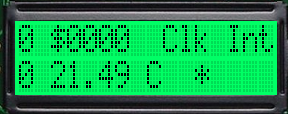
\includegraphics[scale=0.7]{images/dastaZ80_ControlPanel_Page0.png}
        \end{center}

        \begin{itemize}
            \item Line 1:
            \begin{itemize}
                \item \textit{0}: indicates that this is Page 0.
                \item \textit{\$0000}: refers to the address in ROM that will be
                    used to start reading the OS.
                \item \textit{Clk Int}: indicates the the Internal clock is
                    being used as system clock.
            \end{itemize}
            \item Line 2:
            \begin{itemize}
                \item \textit{0}: indicates that this is Page 0.
                \item \textit{21.49 C}: is the current measured internal
                    temperature of the box.
                \item \textit{*}: this only appears if a certain threshold of
                    maximum temperatire has been reached. If the computer is
                    switched ON, here it will appear a spinning animation
                    indicating that the fan is ON. If the computer is OFF, a
                    blinking exclamation mark will appear, indicating that it
                    may not be safe to switch on the computer.
            \end{itemize}
        \end{itemize}

        \textbf{ROM Start Address - Pages 1 and 2}

        Pages 1 and 2 are selectable pages, and show the two different start ROM
        addresses that can be selected.

        The EEPROM that contains the OS can have two different versions. One
        version is burned into the EEPROM at address \texttt{0x0000} and the
        other at \texttt{0x4000}. This is useful for testing new versions or
        even having completely different operating systems.

        \begin{center}
            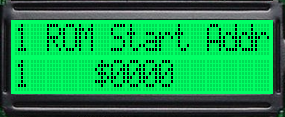
\includegraphics[scale=0.7]{images/dastaZ80_ControlPanel_Page1.png}
            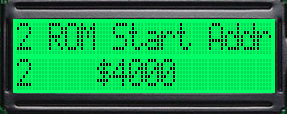
\includegraphics[scale=0.7]{images/dastaZ80_ControlPanel_Page2.png}
        \end{center}

        To select one or the other, press the button \textit{Select} while in
        the desired page. After a couple of seconds, the Panel will display Page
        0 automatically, and you should see the selected value in its
        corresponding position.

        \textbf{System Clock - Pages 3 and 4}

        Pages 3 and 4 are selectable pages, and show the two different system
        clock that can be selected.

        The Internal clock is a 7.3728 Mhz clock, soldered in the Main Board,
        that supplies clock signal to the different devices. The External clock
        is a clock of any speed that can be connected to the
        \textit{External Clock} pin in the box, and will supply the clock signal
        to the different devices.

        The current hardware set up of the dastaZ80DB requires a 7.3728 Mhz
        clock for the serial device to work. Therefore, external clock SHOULD
        only be used for other operating systems than the current version of 
        DZOS.

        \begin{center}
            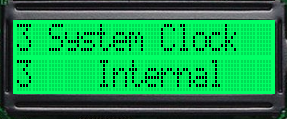
\includegraphics[scale=0.7]{images/dastaZ80_ControlPanel_Page3.png}
            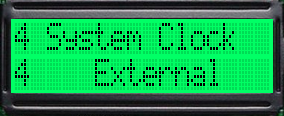
\includegraphics[scale=0.7]{images/dastaZ80_ControlPanel_Page4.png}
        \end{center}

        \textbf{Video Output - Pages 5 and 6}

        Pages 5 and 6 are selectable pages, and show the two different video
        output that can be selected.

        You MUST change this configuration accordingly to how you did set up the
        computer (as explained in the section \hyperref[sec:setting_system]
        {Setting up the system}). Select \textit{TTL Serial} if you are using
        a TTL-to-USB (or TTL-to-RS-232) cable for input and output, or Select 
        \textit{VGA} if you are using TTL-to-USB (or TTL-to-RS-232) cable for
        input but VGA for output.

        \begin{center}
            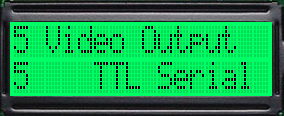
\includegraphics[scale=0.7]{images/dastaZ80_ControlPanel_Page5.png}
            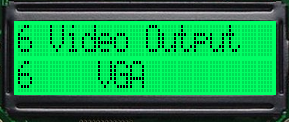
\includegraphics[scale=0.7]{images/dastaZ80_ControlPanel_Page6.png}
        \end{center}

    \pagebreak
    
    % ==========================================================================
    \subsection{ON/OFF button}
    % ==========================================================================
    \label{subsec:onoffbutt}

    The ON/OFF button is located on the lefthand side of the back of the
    dastaZ80 computer and on the front of the dastaZ80DB.

    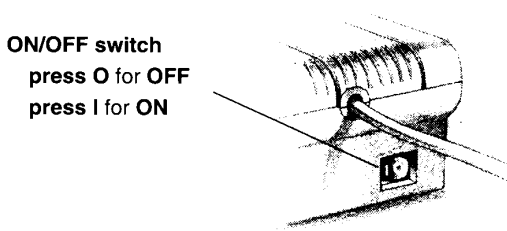
\includegraphics[scale=0.5]{images/onoffbutton.png}

    This button is used to turn ON and OFF the computer.

    Before turning it ON, read the instriuctions on the section
    \hyperref[sec:setting_system]{Setting up the system} of this manual.

    Before turning it OFF, it is highly recommended to use the command 
    \hyperref[cmd:halt]{halt} to ensure that all \textbf{DISK} data has been
    correctly saved. Otherwise, corruption of data may occur.

    % ==========================================================================
    \subsection{Reset button}
    % ==========================================================================
    \label{subsec:resetbutton}

    The reset button is located on the lefthand side of the dastaZ80 computer
    and on the front of the dastaZ80DB.

    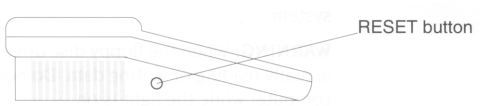
\includegraphics[scale=0.7]{images/resetbutton.png}

    This button is used to restart the computer without turning it off via the
    \hyperref[subsec:onoffbutt]{ON/OFF button}.

    To reset the computer simply press and release the button. The reset process
    will take 6.5 seconds in total, as explained in the section
    \textit{Reset circuit} of the dastaZ80 Technical Reference
    Manual\cite{dastaz80techman}.

    % ==========================================================================
    \subsection{Indicator LEDs}
    % ==========================================================================

    Indicator LEDs for the dastaZ80DB has been discussed in previous section
    \hyperref[subsec:frontpanel]{dastaZ80DB Front Panel}.

    For the dastaZ80, at the top of the computer case there a few labelled
    LEDs that give information of the  status of several internal parts of the
    computer.

    \begin{itemize}
        \item Above the numeric pad, on the righthand side of the keyboard,
        there are two LEDs:
        \begin{itemize}
            \item \textbf{POWER}. This LED is always on when the computer is
            switched on via the \hyperref[subsec:onoffbutt]{ON/OFF button}. It glows
            in \underline{orange} colour.
            \item \textbf{DISC}. This LED blinks whenever a \textbf{DISK} operation
            (read/write) is happening. It glows in \underline{green} colour.
        \end{itemize}
    \end{itemize}
    
    \centerline{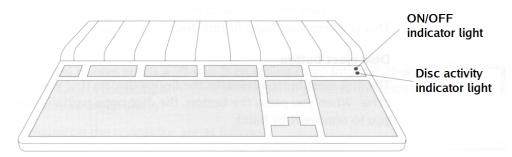
\includegraphics[scale=0.5]{images/keyboardLEDs.png}}

    \begin{itemize}
        \item Above the \textit{Esc} and function keys (\textit{F1}-\textit{F12}),
        on the lefthand side of the keyboard, there are two LEDs. These LEDs are
        multi-colour, hence glowing at different colour each:
        \begin{itemize}
            \item Computer status
            \begin{itemize}
                \item \textbf{RESET}. It glows in \underline{red} colour when
                the computer is in reset status. This happens for 6.5 seconds
                when the computer is switched ON (via the
                \hyperref[subsec:onoffbutt]{ON/OFF button}) and when the
                computer is reset via the \hyperref[subsec:resetbutton]
                {Reset button}.
                \item \textbf{HALTED}. It glows in \underline{blue} when the
                computer is in halt status. Usually after issuing the command
                \hyperref[cmd:halt]{halt}.
                \item \textbf{ROM PAGED}. It glows in \underline{green} when the
                \textbf{ROM} has been electrically disconnected and therefore
                the computer will only perform operations (read/write) from/to
                the \textbf{RAM}. This happens only during the Boot Sequence.
                See the section \textit{OS Boot Sequence} of the dastaZ80
                Programmer's Reference Guide\cite{dastaz80progref} for more
                detailed information about the Boot Sequence.
            \end{itemize}
            \item Clock Selection
            \begin{itemize}
                \item \textbf{CLOCKSEL}. It glows in \underline{yellow} colour
                when the Internal clock is used. And in \underline{purple}
                colour when an External clock is being used by the computer.
            \end{itemize}
        \end{itemize}
    \end{itemize}

    % ==========================================================================
    \subsection{MicroSD}
    % ==========================================================================

    At the back of the dastaZ80 computer and on the front of the dastaZ80DB
    there is a MicroSD slot.

    Insert here a MicroSD formatted with FAT32 and containing Disk Image
    Files formatted with DZFS\footnote{DZFS (dastaZ80 File System) is a file
    system of my own design, for mass storage devices, aimed at simplicity}.

    \centerline{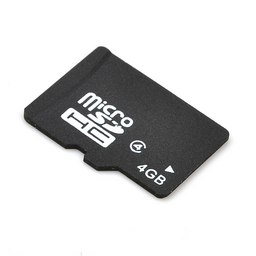
\includegraphics[scale=0.5]{images/microsdcard.png}}

    % ==========================================================================
    \subsection{3.5 inch Floppy Disc Drive}
    % ==========================================================================

    The Floppy Disc Drive is located on the righthand side of the dastaZ80
    computer and on the front of the dastaZ80DB.

    3.5 inch floppy discs can be inserted in this drive. 

    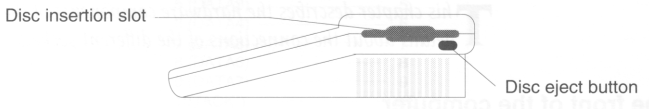
\includegraphics[scale=0.7]{images/discslot.png}

    To remove an inserted floppy disc from the drive, press the
    \textit{Disc eject button}. The disc will partially pop out, allowing you to
    completelly remove it by hand.

    % ==========================================================================
    \subsection{Attaching peripheral devices}
    % ==========================================================================

        % ==========================================================================
        \subsubsection{TTL I/O}
        % ==========================================================================

        The dastaZ80DB has a 4 pins header labelled \textit{TTL I/O} that is
        used to connect either a TTL-to-USB cable or a TTL-to-RS-232 converter.

        This connector carries the signals for the input (keyboard) and output
        (screen).

        By connecting the dastaZ80DB to another computer, the latter can
        \textit{control} the former. As a matter of fact, there is no other way
        to input commands to the dastaZ80DB than using another device (a
        computer in most cases, but also a serial terminal can be used).

        For the output, two options are available:

        \begin{itemize}
            \item \textit{TTL}: output to a serial device (usually another
                computer running a terminal program).
            \item \textit{VGA}: output to a VGA monitor.
        \end{itemize}

        The \textit{TTL / VGA} switch (located on the \hyperref[subsec:frontpanel]
        {Front Panel}) MUST be set up to the correct position, in order to see
        output from the dastaZ80DB.

        The TTL connector pins are configured as follows (seeing it from the
        front):

        \textbf{Ground} | NC | NC | \textbf{TX} | \textbf{RX} | NC

        NC, stands for Not Connected. These are the \textit{+5V}, \textit{/CTS}
        and \textit{/RTS} signals, which are not used.



        % ==========================================================================
        \subsubsection{Dual Video Output}
        % ==========================================================================

        At the back of the computer you will find two connectors, beside each
        other, for the connection of video output.

        The first one, and necessary to use the computer, is a VGA connector for
        the \textbf{VGA video output}.
        
        Plug here a standard VGA cable connected to a VGA monitor.

        \centerline{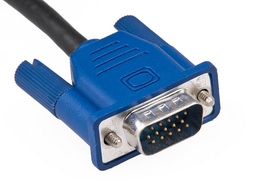
\includegraphics[scale=0.5]{images/vgaconn.png}}

        The second connector, which is optional (i.e. the computer will function
        perfectly normal without this connected), is a 3.5mm female jack for the
        NTSC \textbf{Composite video output}.

        Plug here the jack side of a 3.5mm jack-to-3-RCA Audio/Video cable
        \footnote{This is the same cable used on the Raspberry Pi for Composite
        output.}.

        \centerline{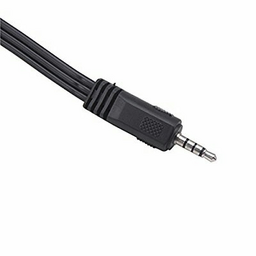
\includegraphics[scale=0.5]{images/raspicable_jack.png}}

        Connect the yellow RCA cable of the jack-to-3-RCA cable to the Composite
        input of a monitor or TV.

        \centerline{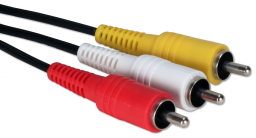
\includegraphics[scale=0.5]{images/raspicable_rca.png}}

        % ==========================================================================
        \subsubsection{Stereo Sound Output}
        % ==========================================================================

        The stereo sound signal comes out of the same connector used for the
        Composite video output.

        Connect the jack-to-3-RCA white and red cables to a pair of speakers or
        to the input of a sound system amplifier.

        % ==========================================================================
        \subsubsection{USB Keyboard for External computer}
        % ==========================================================================

        The keyboard of the dastaZ80 can be used as an USB keyboard on other
        computers.
        
        Connect the a USB cable between this connector and your other
        computer, switch on dastaZ80 and press the key \textit{ScrollLock}. From
        now on (as indicated by the ScrollLock LED being lighted) dastaZ80 will
        not read any keystrokes, but instead will send them to the computer
        connected via USB.

        If you want to use dastaZ80 at any time, just press \textit{ScrollLock}
        again. There is no need to unplug the USB cable. The \textit{ScrollLock}
        key is doing the switching.

        This feature can be handy when you are using dastaZ80 and another PC at
        the same time and don't want to be switching hands between two keyboards
        all the time. It saves space too!

        % ==========================================================================
        \subsubsection{ROM Cartridge}
        % ==========================================================================

        Refer to the section \textit{Cartridge Port} of the dastaZ80 Technical
        Reference Manual\cite{dastaz80techman} for more detailed information.

        % % ==========================================================================
        % \subsubsection{General-Purpose Input/Output (GPIO)}
        % % ==========================================================================

        % This connector exposes all CPU signals and can be used to connect external
        % devices directly to the components (e.g. \textbf{CPU}, \textbf{RAM)} of
        % the computer.
    \pagebreak
    % ==========================================================================
\section{Computer Maintenance}
% ==========================================================================

    % ==========================================================================
    \subsection{Internal Battery}
    % ==========================================================================

    While it is switched off, the computer keeps the date and time, thanks to
    its Real-Time Clock (RTC) internal circuitry.

    This circuitry is supported by a LIR2032 Li-Ion Rechargeable 3.6V Battery
    Button Cell.

    Ideally, to maintain the battery at full charge, the computer SHOULD be
    switched on for at least one hour every month.

    After a few years, due the way rechargeable batteries work, the battery may
    be unable to recharge anymore. In such case, the baterry MUST be replaced
    with a new battery of the same characteristics.

    If you are not planning to use the computer for a year or more, it is highly
    recommended to remove the battery, to avoid leacking of chemical liquids
    that are highly toxic but also can damage the internal circuitry.

    To replace/remove the battery you need to open the computer case. To do so,
    unscrew the three small cross-head screws under the front edge of the
    computer case.

    \centerline{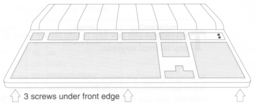
\includegraphics[scale=1]{images/keyboardscrews.png}}

    There is no danger of electrical shock, as the computer is power just by 5V,
    but it is highly recommended to unplug the computer to avoid possible short
    circuits that could damage the internal circuitry. It is also recommened to
    discharge yourself from static electricity before touching the inside of the
    computer.

    % ==========================================================================
    \subsection{Cleaning the computer}
    % ==========================================================================

    In general, avoid high humidity, extreme cold, and extreme heat environments.

    It is highly recommended to use a cover to avoid the concentration of dust
    in the keyboard, which can lead to false contacts.

    Do not put the computer in the dishwasher!
    \pagebreak
    % ==========================================================================
\section{Operating System (OS)}
% ==========================================================================
dzOS (or DZOS) is a single-user single-task ROM-based operating system (OS)
for the 8-bit homebrew computer dastaZ80. It is heavily influenced by ideas
and paradigms coming from Digital Research, Inc. CP/M, so some concepts may
sound familiar to those who had used this operating system.

The user communicates with the OS via a keyboard and a screen connected
directly to the computer.

The main job of dzOS is to allow the user to run programs, one at a time and
communicate with the different peripherals (or devices, as referred in this
manual). The user types in a command and the operating system checks what to
do with the command received, to execute a set of instructions.

Other tasks of dzOS are: handling disk files via its file system (DZFS),
getting user input from the keyboard, writing messages on the screen and
receiving/sending data through the serial port.

dzOS consists of three parts:
\begin{itemize}
    \item The \textbf{BIOS}, that provides functions for controlling the
    hardware.
    \item The \textbf{Kernel}, which provides general functions for
    everything that is not hardware dependent.
    \item The Command-Line Interface (\textbf{CLI}), that provides commands
    for the user to talk to the Kernel and the BIOS.
\end{itemize}

The Kernel and the CLI are hardware independent and will work on other Z80
based computers. Therefore, by adapting the BIOS code, dzOS can easily be
ported to other Z80 systems.

    % ==========================================================================
    \subsection{dastaZ80 File System (DZFS)}
    % ==========================================================================
    A file system manages access to the data stored in a storage medium, a
    SD card in the case of dastaZ80, and allows the OS to load and save data in
    the SD card. From now on, referred as \textbf{DISK}.

    DZFS is my first time designing a file system and for this reason I kept it
    very simple.

    It uses Logical Block Addressing (LBA) for accessing the data on the
    \textbf{DISK}, and an allocation table system based in blocks of sectors.
    The allocation table is called Block Allocation Table (BAT).

    Without entering into much details, bytes in the \textbf{DISK} are organised
    as Sectors, and Sectors are grouped into Blocks. Each Sector is 512 bytes
    long and each Block holds 64 Sectors. Therefore, a Block is 32,768 bytes
    long (64 * 512).

    As the free RAM of dastaZ80 is about 48 KB, it makes no sense to have files
    bigger than that, as it would not fit into \textbf{MEMORY}. Therefore, I
    have decided that each Block can store only a single file.

        % ==========================================================================
        \subsubsection{DZFS limitations}
        % ==========================================================================
        The current version of the DZFS implementation (DZFSV1) have the following
        limitations:

        \begin{itemize}
            \item No support for directories. All files are presented at the same
            level.
            \item Filenames:
            \begin{itemize}
                \item Are case sensitive.
                \item Can be maximum 14 characters long.
                \item Can only contain alphabetical (A to Z) and numerical (0 to 9)
                letters.
                \item Cannot start with a number.
                \item No support for extensions. But there is a separate field for
                File Type.
            \end{itemize}
            \item Maximum size for a file is 32,768 bytes.
        \end{itemize}
        
    % ==========================================================================
    \subsection{The Command Prompt}
    % ==========================================================================
    When you switch ON the computer, you will hear a low tone (beep).

    The \textbf{Low Resolution Display} will display a welcome text and the 
    \textbf{High Resolution Display} will show some information:

    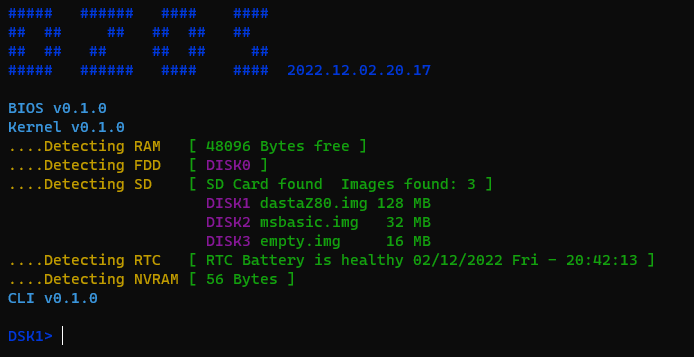
\includegraphics[scale=0.6]{images/dzOS.png}

    This information tells you about the release version of DZOS (2022.07.19.13
    in the screenshot). The BIOS, Kernel and CLI versions, and the detection of
    the different devices used by the computer. It also tells about whichs 
    \textbf{DISK}s are available.

    After that information,you will see the \textit{command prompt}. It starts
    with the letters \textit{DSK} (short for DISK) and a number, followed by the
    symbol $>$

    The number indicates which \textbf{DISK} is currently used for \textbf{DISK}
    operations.

    In other words, if you see \textit{DSK0}, it means that the Floppy Disk Drive
    (\textbf{FDD}) is selected. Entering commands like \textit{cat},
    \textit{diskinfo}, \textit{load}, etc., will instruct the computer to do it
    on the \textbf{FDD}.
    \pagebreak
    % ==========================================================================
\section{OS Commands}
% ==========================================================================
There are a number of commands included in the operating system. These
commands are stored in \textbf{MEMORY} at boot time, and therefore can be
called at any time from the command prompt.

Some commands may have mandatory and/or optional parameters. These
parameters MUST be entered in the order listed. Interchanging the order of
parameters will result on undesired behaviour.

Parameters can be separated either by a comma or a space. For clarity, in
this document all parameters are separated by a comma.

Programs stored in \textbf{DISK} can be executed directly by simply entering
the filename as a command. But only those in the current \textbf{DISK} (see
command \hyperref[cmd:dsk]{dsk}) and with attribute \textit{EXE}.

    % ==========================================================================
    \subsection{General Commands}\label{gencmds}
    % ==========================================================================
        
        % % ======================================================================
        % \subsubsection{{help}}
        % % ======================================================================
        % Shows a list of the most important commands available for the user.
        % For a complete list of commands, refer always to this manual.

        % \hspace{1.9cm}\textbf{$>$ help}

        % \textbf{Parameters}: None

        % ======================================================================
        \subsubsection{{peek}}
        % ======================================================================
        \label{cmd:peek}

        Prints the value of the byte stored at a specified \textbf{MEMORY}
        address.

        \hspace{1.9cm}\textbf{$>$ peek \textit{$<$address$>$}}

        \textbf{Parameters}:

        \hspace{1cm}\textbf{\textit{address}}: address where the user wants
        to get the value from.

        \textbf{Example}: \texttt{$>$ peek 41A0}

        Will print (in hexadecimal) whatever byte is at location 0x41A0.

        % ======================================================================
        \subsubsection{{poke}}
        % ======================================================================
        \label{cmd:poke}

        Changes the value of the byte stored at a specified \textbf{MEMORY}
        address.

        \hspace{1.9cm}\textbf{$>$ poke \textit{$<$address$>$,$<$value$>$}}

        \textbf{Parameters}:

        \hspace{1cm}\textbf{\textit{address}}: address where the user wants
        to change a value.
        
        \hspace{1cm}\textbf{\textit{value}}: new value (in Hexadecimal notation)
        to be stored at \textit{address}.

        \textbf{Example}: \texttt{$>$ poke 41A0,2D}

        Will overwrite the contents of the address 0x41A0 with the value
        0x2D.

        % ======================================================================
        \subsubsection{{autopoke}}
        % ======================================================================
        Allows the user to enter a series of values to be stored at the
        starting address and its consecutive addresses. Think of it like a
        way to do poke but without having to enter the \textbf{MEMORY}
        address each time.

        After entering the command, a different command prompt, denoted by
        the symbol \$, will be displayed.

        Values are entered one by one after the symbol \$. Pressing 
        \textit{Return} with no value will end the command.

        \hspace{1.9cm}\textbf{$>$ autopoke \textit{$<$address$>$}}

        \textbf{Parameters}:

        \hspace{1cm}\textbf{\textit{address}}: address where the user wants
        to start changing values.

        \textbf{Example}: \texttt{$>$ autopoke 41A0}

        Will overwrite the contents of the address 0x41A0 with the first
        value entered by the user at the \$ prompt. Next value entered will
        overwrite the contents of the address 0x41A1, next 0x41A2, and so on
        until the end of the command.

        % ======================================================================
        \subsubsection{{halt}}
        % ======================================================================
        \label{cmd:halt}
        
        Tells the \textbf{DISK} controller to close all files, disables
        interrupts and puts the CPU in halted state, effectively making the
        computer unusable until next power cycle (\textit{Have you tried turning
        it off and on again?}).

        SHOULD be used before switching the computer off, to ensure all
        \textbf{DISK} data has been correctly saved. MUST not be used while the
        busy light of the \textbf{DISK} is on.

        \hspace{1.9cm}\textbf{$>$ halt}

        \textbf{Parameters}: None

        % ======================================================================
        \subsubsection{{run}}
        % ======================================================================
        \label{cmd:run}

        Transfers the Program Counter (PC) of the Z80 to the specified address.
        In other words, this command is used to directly run code that has been
        already loaded in \textbf{RAM}, for example with the command 
        \hyperref[cmd:load]{load}.

        \hspace{1.9cm}\textbf{$>$ run \textit{$<$address$>$}}

        \textbf{Parameters}:

        \hspace{1cm}\textbf{\textit{address}}: address from where to start
        running.
        
        \textbf{Example}: \texttt{$>$ run 4420}

        The \textbf{CPU} will start running whatever instructions finds from
        \texttt{0x4420} and onwards. Programs run this way MUST end with a
        jump instruction (JP) to CLI prompt address, as described in the
        \textit{dastaZ80 Programmer’s Reference Guide}\cite{dastaz80progref}.
        Otherwise the user will have to reset the computer to get back to CLI.
        Not harmful but cumbersome.

        % ======================================================================
        \subsubsection{{crc16}}
        % ======================================================================
        Generates a CRC-16/BUYPASS1\footnote{A 16-bit cyclic redundancy
        check (CRC) based on the IBM Binary Synchronous Communications
        protocol\cite{ibmbsc} (BSC or Bisync). It uses the polynomial
        $X^{16} + X^{15} +X^2 + 1$}

        There are two formats of this command: 
        
        \textbf{crc16 \textit{$<$start\_address$>$ $<$end\_address$>$}}
        and \textbf{crc16 \textit{$<$filename$>$}} 
        
        Here the former is described. See the section \textit{\ref{dskcmds} 
        DISK Commands} on page \pageref{dskcmds} for the other format.

        \hspace{1.9cm}\textbf{$>$ crc16 \textit{$<$start\_address$>$
        $<$end\_address$>$}}
        
        \textbf{Parameters}:

        \hspace{1cm}\textbf{\textit{start\_address}}: first address from
        where the bytes to calculate the CRC will be read.

        \hspace{1cm}\textbf{\textit{end\_address}}: last address from where
        the bytes to calculate the CRC will be read.

        \textbf{Example}: \texttt{$>$ crc16 0000,0100}

        Will calculate the CRC of all bytes in MEMORY between the two
        specified address and show it on the screen:
        
        \hspace{1cm}\texttt{CRC16:\ 0x2F25}

        % ======================================================================
        \subsubsection{{clrram}}
        % ======================================================================
        Fills with zeros the entire Free RAM area (i.e. from 0x4420 to
        0xFFFF).

        \hspace{1.9cm}\textbf{$>$ clrram}

        \textbf{Parameters}: None

    % ======================================================================
    \subsection{Real-Time Clock (RTC) Commands}
    % ======================================================================
        % ======================================================================
        \subsubsection{{date}}
        % ======================================================================
        Shows the current date and day of the week from the Real-Time Clock
        (\textbf{RTC}).

        \hspace{1.9cm}\textbf{$>$ date}

        \textbf{Parameters}: None

        Will show (will differe depending on the date on the \textbf{RTC}):

        \hspace{1cm}\texttt{Today:\ 22/11/2022 Tue}

        % ======================================================================
        \subsubsection{{time}}
        % ======================================================================
        Shows the current time from the Real-Time Clock (\textbf{RTC}).

        \hspace{1.9cm}\textbf{$>$ time}

        \textbf{Parameters}: None

        Will show (will differe depending on the time on the \textbf{RTC}):

        \hspace{1cm}\texttt{Now:\ 16:24:36}

        % ======================================================================
        \subsubsection{{setdate}}
        % ======================================================================
        Changes the current date stored in the Real-Time Clock (\textbf{RTC}).

        \hspace{1.9cm}\textbf{$>$ setdate \textit{$<$yy$>$$<$mm$>$$<$dd$>$$<$dow$>$}}

        \textbf{Parameters}:

        \hspace{1cm}\textbf{\textit{yy}}: year.

        \hspace{1cm}\textbf{\textit{mm}}: month.

        \hspace{1cm}\textbf{\textit{dd}}: day.

        \hspace{1cm}\textbf{\textit{dow}}: day of the Week. (1=Sunday).

        \textbf{Example}: \texttt{$>$ setdate 2211032}

        % ======================================================================
        \subsubsection{{settime}}
        % ======================================================================
        Changes the current time stored in the Real-Time Clock (\textbf{RTC}).

        \hspace{1.9cm}\textbf{$>$ settime \textit{$<$hh$>$$<$mm$>$$<$ss$>$}}

        \textbf{Parameters}:

        \hspace{1cm}\textbf{\textit{hh}}: hour.

        \hspace{1cm}\textbf{\textit{mm}}: minutes.

        \hspace{1cm}\textbf{\textit{ss}}: seconds.

        \textbf{Example}: \texttt{$>$ settime 185700}

    % ==========================================================================
    \subsection{Disk Commands}\label{dskcmds}
    % ==========================================================================
        % ======================================================================
        \subsubsection{{cat}}
        % ======================================================================
        \label{cmd:cat}

        Shows a catalogue of the files stored in the \textbf{DISK}.

        \hspace{1.9cm}\textbf{$>$ cat}

        \textbf{Parameters}: None

        \textbf{Example}: \texttt{$>$ cat}

        Will show (will differ depending on the contents of your \textbf{DISK}):

        \texttt{
        \resizebox{12cm}{!}{
            \begin{tabular}{l l l l l l}
                \multicolumn{6}{l}{Disk Catalogue}\\
                \multicolumn{6}{l}{----------------------------------------------------------------------}\\
                File & Type & Last Modified & Load Address & Attributes & Size\\
                \multicolumn{6}{l}{----------------------------------------------------------------------}\\
                HelloWorld & EXE & 12-03-2022 13:21:44 & 4420 & R SE & 38\\
                file2 & TXT & 11-05-2022 17:12:45 & 0000 & SE & 241
            \end{tabular}
        }}

        \hfill\break

        By default, deleted files are not shown in the catalogue. To show also
        deleted files do a \textit{poke 40ac, 01}. And a \textit{poke 40ac, 00}
        to hide them again.

        Deleted files are identified by a \textasciitilde symbol in the first
        character of the filename.

        \texttt{
        \resizebox{12cm}{!}{
            \begin{tabular}{l l l l l l}
                \multicolumn{6}{l}{Disk Catalogue}\\
                \multicolumn{6}{l}{----------------------------------------------------------------------}\\
                File & Type & Last Modified & Load Address & Attributes & Size\\
                \multicolumn{6}{l}{----------------------------------------------------------------------}\\
                \textasciitilde elloWorld & EXE & 12-03-2022 13:21:44 & 4420 & R SE & 38\\
                file2 & TXT & 11-05-2022 17:12:45 & 0000 & SE & 241
            \end{tabular}
        }}

        \hfill\break

        % ======================================================================
        \subsubsection{{erasedsk}}
        % ======================================================================
        Overwrittes all bytes of all sectors in a \textbf{DISK} in the
        \textbf{FDD}, with \texttt{0xF6} \\

        \underline{This is a destructive action} and it makes the \textbf{DISK}
        unusable to any (included dzOS) computer, as there is no file system in
        the disk after the command is completed.
        
        Before it can be used by dzOS, the command \textit{formatdsk} MUST be
        executed.

        It is recommended to only use this command in the case of wanting to
        destroy all data in a \textbf{DISK}, because \textit{formatdsk} doesn't
        actually delete any data, or to check if a Floppy Disk is faulty.
        Otherwise, the command \textit{formatdsk} SHOULD be the right command
        for normal usage of the computer.

        \hspace{1.9cm}\textbf{$>$ erasedsk}

        \textbf{Parameters}: None

        \textbf{Example}: \texttt{$>$ erasedsk}

        % ======================================================================
        \subsubsection{{formatdsk}}
        % ======================================================================
        Formats a \textbf{DISK} with DZFS format. \underline{This is a
        destructive action} and makes the \textbf{DISK} unsuable by any
        computers not using DZFS as their file system. It overwrites the DZFS
        \textit{Superblock} and \textit{BAT}.

        \hspace{1.9cm}\textbf{$>$ formatdsk \textit{$<$label$>$}}

        \textbf{Parameters}:

        \hspace{1cm}\textbf{\textit{label}}: a name given to the \textbf{DISK}.
        Useful for identifying different disks. It can contain any characters,
        with a maximum of 16.

        \textbf{Example}: \texttt{$>$ formatdsk mainDisk}

        Will format the SD card inserted in the SD card slot at the back of the
        computer case, having \textit{mainDisk} as disk label.

        % ======================================================================
        \subsubsection{{load}}
        % ======================================================================
        \label{cmd:load}

        Loads a file from \textbf{DISK} to \textbf{RAM}.
        
        The file will be loaded in \textbf{RAM} at the address from which it was
        originally saved. This address is stored in the DZFS BAT and cannot be
        changed. 

        \hspace{1.9cm}\textbf{$>$ load \textit{$<$filename$>$}}

        \textbf{Parameters}:

        \hspace{1cm}\textbf{\textit{filename}}: the name of the file that is to
        be loaded.

        \textbf{Example}: \texttt{$>$ load HelloWorld}

        Will load the contents (bytes) of the file \textit{HelloWorld} and copy
        them into the \textbf{RAM} address from which it was originally saved.

        % ======================================================================
        \subsubsection{{rename}}
        % ======================================================================
        Changes the name of a file.

        \hspace{1.9cm}\textbf{$>$ rename \textit{$<$current\_filename$>$,
        $<$new\_filename$>$}}

        \textbf{Parameters}:

        \hspace{1cm}\textbf{\textit{current\_filename}}: the name of the file as
        existing in the \textbf{DISK} at the moment of executing this command.
        
        \hspace{1cm}\textbf{\textit{new\_filename}}: the name that the file will
        have after the command is executed.

        \textbf{Example}: \texttt{$>$ rename HelloWorld,Hello}

        Will change the name of the file \textit{HelloWorld} to \textit{Hello}.

        % ======================================================================
        \subsubsection{{delete}}
        % ======================================================================
        Deletes a file from the \textbf{DISK}.

        Technically is not deleting anything but just changing the first
        character of the filename to a \textasciitilde symbol, which makes it to
        not show up with the command \textit{cat}. Hence, it can be undeleted by
        simply renaming the file. But be aware, when saving new files DZFS looks
        for a free space \footnote{By free space on the \textbf{DISK} we
        understand a Block in the DZFS BAT that was never used before by a
        file.} on the \textbf{DISK}, but if it does not find any it starts
        re-using space from files marked as deleted and hence overwriting data
        on the \textbf{DISK}.

        \hspace{1.9cm}\textbf{$>$ delete \textit{$<$filename$>$}}

        \textbf{Parameters}:

        \hspace{1cm}\textbf{\textit{filename}}: the name of the file that is to
        be deleted.
        
        \textbf{Example}: \texttt{$>$ delete HelloWorld}

        Will delete the file \textit{HelloWorld}.

        % ======================================================================
        \subsubsection{{chgattr}}
        % ======================================================================
        \label{cmd:chgattr}

        Changes the \hyperref[subsub:fileattr]{File Attributes} of a file.

        \hspace{1.9cm}\textbf{$>$ chgattr \textit{$<$filename$>$,$<$RHSE$>$}}

        \textbf{Parameters}:

        \hspace{1cm}\textbf{\textit{filename}}: the name of the file to change
        the attributes.

        \hspace{1cm}\textbf{\textit{RHSE}}: the new attributes (see list above)
        that are to be set to the specified file. Attributes are actually not
        changed but re-assigned. For example, if you have a file with attribute
        \textit{R} and specified only \textit{E}, it will change from Read Only
        to Executable. In order to keep both, you MUST specify both values,
        \textit{RE}.
        
        \textbf{Example}: \texttt{$>$ chgattr HelloWorld,RE}

        Will set the attributes of the the file \textit{HelloWorld} to Read Only
        and Executable.

        % ======================================================================
        \subsubsection{{save}}
        % ======================================================================
        \label{cmd:save}

        Saves the bytes of specified \textbf{MEMORY} addresses to a new file in
        the \textbf{DISK}.

        \hspace{1.9cm}\textbf{$>$ save \textit{$<$start\_address$>$,
        $<$number\_of\_bytes$>$}}

        \textbf{Parameters}:

        \hspace{1cm}\textbf{\textit{$<$start\_address$>$}}: first address where
        the bytes that the user wants to save are located in \textbf{MEMORY}.

        \hspace{1cm}\textbf{\textit{$<$number\_of\_bytes$>$}}: total number of
        bytes, starting at \textit{start\_address} that will be saved to
        \textbf{DISK}.
        
        \textbf{Example}: \texttt{$>$ save 4420,512}

        Will create a new file, with the name entered by the user when prompted,
        with 512 bytes of the contents of \textbf{MEMORY} from 0x4420 to 0x461F.

        % ======================================================================
        \subsubsection{{dsk}}
        % ======================================================================
        \label{cmd:dsk}

        Changes current disk for all \textbf{DISK} operations.

        \hspace{1.9cm}\textbf{$>$ dsk \textit{$<$n$>$}}

        \textbf{Parameters}:

        \hspace{1cm}\textbf{\textit{$<$n$>$}}: \textbf{DISK} number.

        \textbf{Example}: \texttt{$>$ dsk 0}

        Will change to \textbf{FDD}, and all the \textbf{DISK} operations will
        be performed in the \textbf{FDD} until the next boot or a new \textit{dsk}
        command.

        The CLI prompt changes to indicate which disk is in use.

        % ======================================================================
        \subsubsection{{diskinfo}}
        % ======================================================================
        Shows some information about the \textbf{DISK}.

        \hspace{1.9cm}\textbf{$>$ diskinfo}

        \textbf{Parameters}: None

        \textbf{Example}: \texttt{$>$ diskinfo}

        Will show (will differ depending on the contents of your \textbf{DISK}):

        \texttt{
        \resizebox{12cm}{!}{
            \begin{tabular}{l r l l}
                \multicolumn{4}{l}{Disk Information}\\
                & Volume .\ .\ : & dastaZ80 Main & (S/N: 352A15F2)\\
                & File System: & DZFSV1 &\\
                & Created on : & 03/10/2022 14:22:32 &\\
                & Partitions : & 01 &\\
                & Bytes per Sector: & 512 &\\
                & Sectors per Block: & 64 &
            \end{tabular}
        }}

        % ======================================================================
        \subsubsection{{disklist}}
        % ======================================================================
        Shows a list of all available \textbf{DISK} (\textbf{FDD} and Disk Image
        Files on the \textbf{SD}).

        \hspace{1.9cm}\textbf{$>$ disklist}

        \textbf{Parameters}: None

        \textbf{Example}: \texttt{$>$ disklist}

        Will show (will differ depending on the Disk Image Files on your
        \textbf{DISK}):

        \texttt{
        \resizebox{6cm}{!}{
            \begin{tabular}{l l l r}\\
                & DISK0 & FDD & \\
                & DISK1 & dastaZ80.img & 128 MB \\
                & DISK2 & msbasic.img   & 32 MB \\
                & DISK3 & empty.img     & 16 MB
            \end{tabular}
        }}

        \hfill\break

        \textbf{IMPORTANT}: When the list (210 bytes in total, for a maximum of
        15 Disk Image Files) is retrieved from the \textbf{ASMDC}, dzOS stores
        it at the very bottom of the RAM (\texttt{0xFF2D}). In case that you may
        have a program loaded that uses those low bytes, after executing the
        \textit{disklist} command the program will be corrupted.

        % % ======================================================================
        % \subsubsection{{crc16}}
        % % ======================================================================
        % Generates a CRC-16/BUYPASS1\footnote{A 16-bit cyclic redundancy
        % check (CRC) based on the IBM Binary Synchronous Communications
        % protocol (BSC or Bisync). It uses the polynomial
        % $X^{16} + X^{15} +X^2 + 1$}

        % There are two formats of this command: 
        
        % \textbf{crc16 \textit{$<$start\_address$>$ $<$end\_address$>$}}
        % and \textbf{crc16 \textit{$<$filename$>$}} 
        
        % Here the latter is described. See the section \textit{\ref{gencmds} 
        % General Commands} on page \pageref{gencmds} for the other format.

        % \hspace{1.9cm}\textbf{$>$ crc16 \textit{$<$filename$>$}}
        
        % \textbf{Parameters}:

        % \hspace{1cm}\textbf{\textit{filename}}: the name of the file for which
        % the CRC will be calculated.

        % \textbf{Example}: \texttt{$>$ crc16 HelloWorld}

        % Will calculate the CRC of all bytes on the file and show it on the
        % screen:
        
        % \hspace{1cm}\texttt{CRC16:\ 0x3ABC}

    % ==========================================================================
    \subsection{VDP (\textit{Low Resolution Screen}) Commands}\label{vdpcmds}
    % ==========================================================================
        % ======================================================================
        \subsubsection{{vpoke}}
        % ======================================================================
        \label{cmd:vpoke}

        Changes the value of the byte stored at a specified \textbf{VRAM}
        address.

        \hspace{1.9cm}\textbf{$>$ vpoke \textit{$<$address$>$,$<$value$>$}}

        \textbf{Parameters}:

        \hspace{1cm}\textbf{\textit{address}}: address where the user wants
        to change a value.
        
        \hspace{1cm}\textbf{\textit{value}}: new value (in Hexadecimal notation)
        to be stored at \textit{address}.

        \textbf{Example}: \texttt{$>$ vpoke 3800,00}

        Will overwrite the contents of the address 0x3800 of the \textbf{VRAM}
        with the value 0x00.

        % ======================================================================
        \subsubsection{{screen}}
        % ======================================================================
        Changes the \textbf{Low Resolution Screen} display mode.

        \hspace{1.9cm}\textbf{$>$ screen \textit{$<$mode$>$}}

        \textbf{Parameters}:

        \hspace{1cm}\textbf{\textit{mode}}: one of the valid
        \hyperref[sec:vdpscrmodes]{\textbf{Low Resolution} Screen Modes}:

        \begin{itemize}
            \item \textbf{0}: \textbf{Text Mode}.
            \item \textbf{1}: \textbf{Graphics I Mode}.
            \item \textbf{2}: \textbf{Graphics II Mode}.
            \item \textbf{3}: \textbf{Multicolour Mode}.
            \item \textbf{4}: \textbf{Graphics II Mode Bitmapped}.
        \end{itemize}
        
        \textbf{Example}: \texttt{$>$ screen 0}

        Will put the \textbf{Low Resolution Screen} in Text Mode.

        % ======================================================================
        \subsubsection{{clsvdp}}
        % ======================================================================
        Clears the contents of the \textbf{Low Resolution Screen}.

        \hspace{1.9cm}\textbf{$>$ clsvdp}

        \textbf{Parameters}: None
    \pagebreak
    % ==========================================================================
\section{Other Software}
% ==========================================================================

    % ======================================================================
    \subsection{Memory Dump (memdump)}
    % ======================================================================
    \label{software:memdump}

    This program shows the contents (bytes) of a specified range of
    \textbf{MEMORY}.

    The contents are printed as hexadecimal bytes, in groups of 16 per each line
    and with the printable ASCII value (if printable) or just a dot (if not
    printable).

    At the start of the program, the user will be asked to enter the
    \textit{Start Address} and the \textit{End Address}. In the case of leaving
    blank (i.e. just press the \textit{Return} key without entering any value),
    the program will terminate.

    Example for \textit{Start Address} = 0B40 and \textit{End Address} = 0BEF:

    \texttt{
    \resizebox{12cm}{!}{
        \begin{tabular}{l l l l l l l l l l l l l l l l l l}
                    & 00 & 01 & 02 & 03 & 04 & 05 & 06 & 07 & 08 & 09 & 0A & 0B & 0C & 0D & 0E & 0F   & \\
            \cline{2-17}
            0B40: & FF & FF & FF & FF & FF & FF & FF & FF & FF & FF & FF & FF & FF & FF & FF & 00   & ................\\
            0B50: & 21 & 3A & 0F & CD & BE & 03 & 06 & 01 & CD & 20 & 04 & CD & 4D & 0C & 21 & 56   & !:.......\ ..M.!V\\
            0B60: & 0F & CD & BE & 03 & 21 & C4 & 22 & 3E & 00 & 32 & C4 & 22 & CD & 75 & 0B & CD   & ....!.">.2.".u..\\
            0B70: & B1 & 0B & C3 & 5B & 0B & CD & C8 & 03 & FE & 20 & CA & 91 & 0B & FE & 2C & CA   & ...$[$.....\ ....,.\\
            0B80: & 91 & 0B & FE & 0D & CA & B0 & 0B & 77 & 23 & C3 & 75 & 0B & C9 & 2B & C3 & 75   & .......w\#.u..+.u\\
            0B90: & 0B & 3A & E4 & 22 & FE & 00 & CA & A4 & 0B & 3A & 04 & 23 & FE & 00 & CA & AA   & .:.".....:.\#....\\
            0BA0: & 0B & C3 & 75 & 0B & 21 & E4 & 22 & C3 & 75 & 0B & 21 & 04 & 23 & C3 & 75 & 0B   & ..u.!.".u.!.\#.u.\\
            0BB0: & C9 & 21 & C4 & 22 & 7E & FE & 00 & CA & 5B & 0B & 11 & 29 & 14 & CD & 02 & 0C   & .!."~...$[$..$)$....\\
            0BC0: & CA & 89 & 0E & 11 & 10 & 14 & CD & 02 & 0C & CA & 93 & 0E & 11 & 2C & 14 & CD   & .............,..\\
            0BD0: & 02 & 0C & CA & 55 & 0E & 11 & 25 & 14 & CD & 02 & 0C & CA & 15 & 0F & 11 & 15   & ...U..\%.........\\
            0BE0: & 14 & CD & 02 & 0C & CA & 9A & 0E & 11 & 1A & 14 & CD & 02 & 0C & CA & C7 & 0E   & ................
        \end{tabular}
    }}

    If the information reaches the bottom of the screen, a message will be shown
    to let the user decide what to do next:

    \hspace{1cm}\texttt{[SPACE] for more or another key to stop}

    % ======================================================================
    \subsection{Video Memory Dump (vramdump)}
    % ======================================================================
    \label{software:vramdump}

    This program shows the contents (bytes) of a specified range
    of \textbf{VRAM}.

    The contents are printed as hexadecimal bytes, in groups of 16 per each
    line.

    At the start of the program, the user will be asked to enter the
    \textit{Start Address} and the \textit{End Address}. In the case of leaving
    blank (i.e. just press the \textit{Return} key without entering any value),
    the program will terminate.

    Example for \textit{Start Address} = 0000 and \textit{End Address} = 00AF:

    \texttt{
    \resizebox{12cm}{!}{
        \begin{tabular}{l l l l l l l l l l l l l l l l l l}
                    & 00 & 01 & 02 & 03 & 04 & 05 & 06 & 07 & 08 & 09 & 0A & 0B & 0C & 0D & 0E & 0F   & \\
            \cline{2-17}
            0000: & 00 & 00 & 00 & 00 & 00 & 00 & 00 & 00 & FF & FF & FF & FF & FF & FF & FF & FF\\
            0010: & 00 & 00 & 00 & 00 & 00 & 01 & 03 & 07 & 00 & 00 & 00 & 00 & 00 & 80 & C0 & E0\\
            0020: & 07 & 03 & 01 & 00 & 00 & 00 & 00 & 00 & E0 & C0 & 80 & 00 & 00 & 00 & 00 & 00\\
            0030: & F0 & F0 & F0 & F0 & 00 & 00 & 00 & 00 & F0 & F8 & FC & FE & FF & FF & FF & FF\\
            0040: & 0F & 1F & 3F & 7F & FF & FF & FF & FF & FF & FF & FF & FF & FE & FC & F8 & F0\\
            0050: & FF & FF & FF & FF & 7F & 3F & 1F & 0F & 00 & 00 & 00 & 00 & 00 & 00 & 00 & 00\\
            0060: & 0B & C3 & 75 & 0B & 21 & E4 & 22 & C3 & 75 & 0B & 21 & 04 & 23 & C3 & 75 & 0B\\
            0070: & C9 & 21 & C4 & 22 & 7E & FE & 00 & CA & 5B & 0B & 11 & 29 & 14 & CD & 02 & 0C\\
            0080: & CA & 89 & 0E & 11 & 10 & 14 & CD & 02 & 0C & CA & 93 & 0E & 11 & 2C & 14 & CD\\
            0090: & 02 & 0C & CA & 55 & 0E & 11 & 25 & 14 & CD & 02 & 0C & CA & 15 & 0F & 11 & 15\\
            00A0: & 14 & CD & 02 & 0C & CA & 9A & 0E & 11 & 1A & 14 & CD & 02 & 0C & CA & C7 & 0E
        \end{tabular}
    }}

    If the information reaches the bottom of the screen, a message will be shown
    to let the user decide what to do next:

    \hspace{1cm}\texttt{[SPACE] for more or another key to stop}

    % ======================================================================
    \subsection{Load Screen dumps (loadscr)}
    % ======================================================================
    \label{sub:loadscr}
    This program loads screen dumps, saved as raw data, to the the VRAM. It is
    in essence a picture display program.

    In Mode 2 (Graphics II Mode bitmapped), screen data dumps are files of
    14,336 bytes in length, composed by:
    \begin{itemize}
        \item Dump of the Pattern Table (6,144 bytes)
        \item Dump of the Sprite Pattern Table (2,048 bytes) filled with zeros
        \item Dump of the Colour Table (6,144 bytes)
    \end{itemize}

    In dzOS, these files are identified as File Type \textit{SC1}
    (Graphics I Mode), \textit{SC2} (Graphics II Bitmapped Mode) and
    \textit{SC3} (Multicolour Mode).

    % ======================================================================
    \subsection{Load Font (loadfont)}
    % ======================================================================
    \label{sub:loadfont}

    This program loads font files, which contain pattern definitions for text
    characters to be used for text display.

    Mode 0 (Text Mode) uses 6x8 bytes characters. The rest of the modes use 8x8
    bytes characters.

    In dzOS, these files are identified as File Type \textit{FN6} and
    \textit{FN8} respectively.

    % ==========================================================================
    \subsection{MS BASIC 4.7b}
    % ==========================================================================
    \label{sub:msbasic}

    The Nascom 2 computer\footnote{The Nascom 2 was a single-board computer kit
    issued in the United Kingdom in December 1979.} came with MS BASIC 7.4
    installed in ROM, and the disassembled code was published in the
    \textit{80-BUS NEWS} magazine \cite{80busnews23}, \cite{80busnews24},
    \cite{80busnews25}, \cite{80busnews26}, \cite{80busnews31},
    \cite{80busnews32}, \cite{80busnews33}.

    Grant Searle published a modification in his Grant's \textit{7-chip Z80
    computer} webpage\cite{searle2}.

    Grant's version was then modified to run on dastaZ80 under dzOS, adding
    commands like \textit{LOAD}, \textit{SAVE}, \textit{VPOKE}, \textit{VPEEK},
    and more.

        % ==========================================================================
        \subsubsection{MS BASIC characteristics}
        % ==========================================================================

        \begin{itemize}
            \item Commands
            \begin{itemize}
                \item There is no support for \textit{ELSE} in \textit{IF}...
                \textit{THEN}. Instead, it MUST be done with another \textit{IF}...
                \textit{THEN}.
            \end{itemize}
            \item Variables
            \begin{itemize}
                \item The first character of a variable name MUST be a letter.
                \item No reserved words may appear as as variable names.
                \item Can be of any length,, but any alphanumeric characters after
                the first two are ignored. Therefore \textit{COURSE},
                \textit{COLOUR} and\textit{COMIC} are the same variable.
                \item Integer numbers are signed (i.e. from -32,768 to +32,767). To
                refer to a location \textit{n} above 32,767, you must provide the
                2's complement number (i.e \textit{n}-65536)
                \item Flotaing point is in the range 1.70141E38 to 2.9387E-38
            \end{itemize}
        \end{itemize}

        % ==========================================================================
        \subsubsection{Speeding up programs}
        % ==========================================================================

        \begin{itemize}
            \item Delete \textit{REM} statements.
            \item Delete spaces. For example, \textit{10FORA=0TO10} is faster than
            \textit{10 FOR A=0 TO 10}
            \item Use \textit{NEXT} without the index variable.
            \item Use variables instead of constants, especially in \textit{FOR}
            loop and other code that is executed repeatedly.
            \item Reuse variable names and keep the list of variables as short as
            possible. Variables are set up in a table in the order of their first
            appearance in the program. Later in the program, BASIC searches the
            table for the variable at each reference. Variables at the head of the
            table take less time to search.
            \item MS BASIC uses a \textit{garbage collector} to clear out unwanted 
            space. The frequency of grabage collection is inversely proportional to
            the amount of string space. The time garbage collection takes is
            proportional to the square of the number of string variables. To
            minimise the time, make string space as large as possible and use as few
            string variables as possible.
        \end{itemize}

    % ==========================================================================
    \subsection{MS BASIC 4.7b Standard version}
    % ==========================================================================

    Standard version is referring to the version (\textit{b}) adapted by Grant
    Searle \cite{searle1} of the original NASCOM 2 version (4.7).

    For more detailed information on commands, statements, functions, etc.,
    refer to the Nascom 2 Microcomputer BASIC Programming Manuals\cite{nascombasic}.

        % ==========================================================================
        \subsubsection{Intrinsic Functions}
        % ==========================================================================

        \begin{itemize}
            \item \textbf{ABS}: Returns absolute value of a number.
            \item \textbf{ASC}: Returns the ASCII code of the first character of a string.
            \item \textbf{ATN}: Returns arctangent in radians.
            \item \textbf{CHR\$}: Returns a string whose one element has its ASCII code.
            \item \textbf{COS}: Returns cosine in radians.
            \item \textbf{EXP}: Returns the mathematical constant \textit{e} (Euler’s number) to the power of a specified number.
            \item \textbf{FRE}: Returns number of bytes in memory not being used by BASIC.
            \item \textbf{INP}: Reads a byte from a port.
            \item \textbf{INT}: Returns the largest integer of a floating number.
            \item \textbf{LEFT\$}: Returns x leftmost characters of a string.
            \item \textbf{LEN}: Returns length of a string.
            \item \textbf{LOG}: Returns natural log of a number.
            \item \textbf{MID\$}: Returns x characters of a string.
            \item \textbf{POS}: Returns present column position of terminal's print head..
            \item \textbf{RIGHT\$}: Returns x rightmost characters of a string.
            \item \textbf{RND}: Returns a random number between 0 and 1.
            \item \textbf{SGN}: Returns 0 or 1 depending on the sign of a number.
            \item \textbf{SIN}: Returns the sine in radians.
            \item \textbf{SPC}: Prints x number of blanks.
            \item \textbf{SQR}: Returns square root of a number.
            \item \textbf{STR\$}: Returns string representation of value of a number.
            \item \textbf{TAB}: Spaces to x position on the terminal.
            \item \textbf{TAN}: Returns tangent in radians.
            \item \textbf{USR}: Calls a user's machine language subroutine.
            \item \textbf{VAL}: Returns numerical value of a string.
        \end{itemize}

        % ==========================================================================
        \subsubsection{Statements}
        % ==========================================================================

        \begin{itemize}
            \item \textbf{DATA}, \textbf{DEEK}, \textbf{DEF}, \textbf{DIM},
            \textbf{DOKE}, \textbf{END}, \textbf{FN}, \textbf{FOR...NEXT...STEP},
            \textbf{GOTO}, \textbf{GOSUB}, \textbf{IF...THEN}, \textbf{INPUT},
            \textbf{LET}, \textbf{LINES}, \textbf{ON...GOTO}, \textbf{ON...GOSUB},
            \textbf{OUT}, \textbf{PEEK}, \textbf{POKE}, \textbf{PRINT},
            \textbf{READ}, \textbf{REM}, \textbf{RESTORE}, \textbf{RETURN},
            \textbf{STOP}, \textbf{WAIT}, \st{\textbf{WIDTH}}\footnote{The
            command \textit{WIDTH} has been removed because it doesn't have any
            use in dastaZ80.}
        \end{itemize}

        % ==========================================================================
        \subsubsection{Commands}
        % ==========================================================================

        \begin{itemize}
            \item \textbf{CLEAR}: Sets all program variables to zero.
            \item \textbf{CLS}: Clears the screen.
            \item \textbf{CONT}: Continues program execution after \textit{Escape}
            key was pressed, or a \textit{STOP} or \textit{END} statement has
            been executed.
            \item \textbf{LIST}: List the contents of the BASIC program in memory.
            \item \textbf{MONITOR}: Transfer command to dzOS Command-Line
            Interface (CLI).
            \item \textbf{NEW}: Deletes the current program and clears all
            variables.
            \item \textbf{NULL}: Sets the number of nulls to be printed at the
            end of each line.
            \item \textbf{RUN}: Starts execution of the current program.
        \end{itemize}

        % ==========================================================================
        \subsubsection{Operators}
        % ==========================================================================

        \begin{itemize}
            \item \textbf{+} Addition
            \item \textbf{-} Subtraction
            \item \textbf{*} Multiplication
            \item \textbf{/} Division
            \item \textbf{\textasciicircum} Power of
        \end{itemize}

        % ==========================================================================
        \subsubsection{Relational Operators}
        % ==========================================================================

        \begin{itemize}
            \item \textbf{$>$}, \textbf{$<$}, \textbf{$<>$}, \textbf{=},
            \textbf{$<=$}, \textbf{$>=$}
        \end{itemize}

        % ==========================================================================
        \subsubsection{Logical Operators}
        % ==========================================================================

        \begin{itemize}
            \item \textbf{AND}, \textbf{NOT}, \textbf{OR}
        \end{itemize}

        % ==========================================================================
        \subsubsection{How to call an ASM subroutine}
        % ==========================================================================

        This BASIC provides a way of executing external subroutines, via the
        intrinsic function \textit{USR}.

        The programmer needs to store the address of the subroutine to be called in
        the the work space location reserved for \textit{USR}. In the case of the
        version for dastaZ80, this is at \texttt{0x6148} for the LSB and
        \texttt{0x6149} for the MSB.

        This can be done from BASIC with the instruction \texttt{DPOKE 24904,<address>}

        \textbf{Be aware} that at location \texttt{0x6147} there is stored a
        \textit{jp} instruction, which is what is executed when the function
        \textit{USR} is called from BASIC, and therefore it will jump to the
        subroutine and never come back unless explicitily specified.

        If instead your subroutine contains a \textit{ret}urn instruction, or if you
        are calling dzOS functions, you \textbf{MUST} change the \textit{jp}
        instruction to a \textit{call} instruction.

        This can be done from BASIC with the instruction \texttt{POKE 24903,205}

        Finally, to call the external subroutine, as the \textit{USR} is a function,
        it returns a parameter and therefore it must be received. Either by assigning
        the value to a variable (e.g. \texttt{A=USR(0)}) or by printing it or by
        checking it with an \textit{IF}.

        \begin{itemize}
            \item Valid methods how to use \textit{USR}:
            \begin{itemize}
                \item \texttt{A=USR(0)}
                \item \texttt{IF USR(0)<>0 THEN ...}
                \item \texttt{PRINT USR(0)}
            \end{itemize}
            \item Invalid methods:
            \begin{itemize}
                \item \texttt{USR(0)}, will return \textit{?SN Error} (i.e. Syntax Error)
            \end{itemize}
        \end{itemize}

    % ==========================================================================
    \subsection{MS BASIC 4.7b dastaZ80 version}
    % ==========================================================================

    In addition to adapting Grant Searle's version to the dastaZ80 computer,
    the following has been added:

        % ======================================================================
        \subsubsection{{CAT}}
        % ======================================================================
        Shows a list of BASIC programs in the current disk. Only files of type
        BASIC are listed, any other files are ignored.

        \hspace{1.9cm}\textbf{CAT}

        \textbf{Parameters}: None

        \textbf{Example}: \texttt{CAT}

        % ======================================================================
        \subsubsection{{COLOUR}}
        % ======================================================================
        Changes the foreground and background colours of the \textbf{Low
        Resolution Display} screen.

        \hspace{1.9cm}\textbf{COLOUR \textit{$<$foreground$>$,$<$background$>$}}

        \textbf{Parameters}:

        \hspace{1cm}\textbf{\textit{$<$foreground$>$}}: number representing one
        of the available VDP colours.

        \hspace{1cm}\textbf{\textit{$<$background$>$}}: number representing one
        of the available VDP colours.

        \textbf{Example}: \texttt{COLOUR 16,4}

        \textbf{Available VDP colours:}

        \begin{itemize}
            \item 0 = Black
            \item 1 = Red
            \item 2 = Green
            \item 3 = Yellow
            \item 4 = Blue
            \item 5 = Magenta
            \item 6 = Cyan
            \item 7 = White
            \item 8 = Bright Black (Grey)
            \item 9 = Bright Red
            \item 10 = Bright Green
            \item 11 = Bright Yellow
            \item 12 = Bright Blue
            \item 13 = Bright Magenta
            \item 14 = Bright Cyan
            \item 15 = Bright White
        \end{itemize}

        % ======================================================================
        \subsubsection{{LOAD}}
        % ======================================================================
        Loads a BASIC program from \textbf{DISK} into \textbf{MEMORY}.

        \hspace{1.9cm}\textbf{LOAD "\textit{$<$filename$>$}}

        \textbf{Parameters}:

        \hspace{1cm}\textbf{\textit{$<$filename$>$}}: the name of the file to be
        loaded.

        \textbf{Example}: \texttt{LOAD "mandelbrot}

        % ======================================================================
        \subsubsection{{SAVE}}
        % ======================================================================
        Saves current BASIC program from \textbf{MEMORY} into current
        \textbf{DISK}.

        \hspace{1.9cm}\textbf{SAVE "\textit{$<$filename$>$}}

        \textbf{Parameters}:

        \hspace{1cm}\textbf{\textit{$<$filename$>$}}: the name of the file to be
        saved.

        \textbf{Example}: \texttt{SAVE "mandelbrot}

        \textbf{Hint}: Although there isn't an MS BASIC command to change the
        current \textbf{DISK}, it can easily be changed manually. DZOS
        \textbf{DISK} operations are performed to whatever \textbf{DISK} number
        is stored in an area of \textbf{MEMORY} called \textit{SYSVARS}
        (See \textit{dastaZ80 Manual - Programmer’s Reference Guide} for more
        details). The \textbf{DISK} number is stored at address \texttt{0x4176},
        therefore by changing the value stored at this address we are
        effectively changing the current \textbf{DISK}. To change it simply use
        \texttt{POKE \&h4176,$<$disknum$>$} where \textit{$<$disknum$>$} is a
        valid \textbf{DISK} number.

        % ======================================================================
        \subsubsection{{SCREEN}}
        % ======================================================================
        Changes the \textbf{Low Resolution Display} screen mode.

        \hspace{1.9cm}\textbf{SCREEN \textit{$<$screen\_mode$>$}}

        \textbf{Parameters}:

        \hspace{1cm}\textbf{\textit{$<$screen\_mode$>$}}: one of the valid
        \hyperref[sec:vdpscrmodes]{\textbf{Low Resolution} Screen Modes}:

        \begin{itemize}
            \item 0 = Text Mode
            \item 1 = Graphics I Mode
            \item 2 = Graphics II Mode
            \item 3 = Multicolour Mode
            \item 4 = Graphics II Mode Bitmapped
        \end{itemize}

        \textbf{Example}: \texttt{SCREEN 2}

        % ======================================================================
        \subsubsection{{SPOKE}}
        % ======================================================================
        Writes a value in a specific \textbf{PSG} register.

        \hspace{1.9cm}\textbf{SPOKE \textit{$<$PSG\_register$>$,$<$value$>$}}

        \textbf{Parameters}:

        \hspace{1cm}\textbf{\textit{$<$PSG\_register$>$}}: \textbf{PSG} register
        number (0-13).

        \hspace{1cm}\textbf{\textit{$<$value$>$}}: value to set (0..255).

        \textbf{Example}: \texttt{SPOKE 7,62}

        % ======================================================================
        \subsubsection{{VPEEK}}
        % ======================================================================
        Gets the value at a specific \textbf{VRAM} address.

        \hspace{1.9cm}\textbf{VPEEK \textit{$<$VRAM\_address$>$}}

        \textbf{Parameters}:

        \hspace{1cm}\textbf{\textit{$<$VRAM\_address$>$}}: \textbf{VRAM} address.

        \textbf{Examples}:
        \begin{itemize}
            \item \texttt{PRINT VPEEK(6144)}
            \item \texttt{A=VPEEK(6144)}
        \end{itemize}

        % ======================================================================
        \subsubsection{{VPOKE}}
        % ======================================================================
        Writes a value at a specific \textbf{VRAM} address.

        \hspace{1.9cm}\textbf{VPOKE \textit{$<$VRAM\_address$>$,$<$value$>$}}

        \textbf{Parameters}:

        \hspace{1cm}\textbf{\textit{$<$VRAM\_address$>$}}: \textbf{VRAM} address.

        \hspace{1cm}\textbf{\textit{$<$value$>$}}: value to set (0..255).

        \textbf{Example}: \texttt{VPOKE 6144,171}

    % ==========================================================================
    \subsection{Machine Language Monitor (mlmonitor)}
    % ==========================================================================
    \label{software:mlmonitor}

    The Machine Language Monitor contains many features that will enable you to
    create, modfy and test machine language program and subroutines.

    It allows to assemble code into memory, disassemble memory, inspect memory,
    save memory into disk, and more.

    Once loaded, the monitor program will display a prompt in the form of a
    single dot.

    At this prompt, the user can enter any of the available commands presented
    below. Just bear in mind that all commands, addresses and bytes MUST be
    entered using capital letters. It is highly recommended to activate the
    \textit{Caps Lock} key during the usage of the monitor program.

    Also, all addresses and bytes MUST be entered in hexadecimal notation.

        % ==========================================================================
        \subsubsection{A - Assemble}
        % ==========================================================================

        Purpose: Assemble a line of assembly code.

        Syntax: A \textit{$<$address$>$ $<$mnemonic$>$ $<$operand$>$}

        Example: \texttt{A 2000 LD A,(HL)}

        \hspace{1cm}\textit{$<$address$>$}: a four-digit hexadecimal number indicating
        the location in memory where to place the generated opcode.

        \hspace{1cm}\textit{$<$mnemonic$>$}: a valid Z80 assembly language
        mnemonic (e.g. LD, ADD, CALL, LDIR).

        \hspace{1cm}\textit{$<$operand$>$}: the operand of the mnemonic.

        For a complete list of valid Z80 mnemonics and its operands check the
        \textit{Z80 Family CPU User Manual}\cite{z80manual}, publiched by ZiLOG.

        % ==========================================================================
        \subsubsection{C - Call}
        % ==========================================================================

        Purpose: Transfers the Program Counter (PC) of the Z80 to the specified
        address. Hence, the \textbf{CPU} starts executing the code it finds at
        the specified address. Works same as the \hyperref[cmd:run]{run} command.

        Syntax: C \textit{$<$address$>$}

        Example: \texttt{C 4000}

        \hspace{1cm}\textit{$<$address$>$}: a four-digit hexadecimal number
        indicating the location in \textbf{RAM} memory of the byte that will be
        displayed.

        \textbf{IMPORTANT}: In order for the \hyperref[software:mlmonitor]
        {Machine Language Monitor} to continue to work after the called
        subroutine ends, the subroutine MUST end with a return (\textit{RET})
        instruction. mlmonitor already takes care of putting in the Stack the
        current address before changing the Program Counter (PC).

        % ==========================================================================
        \subsubsection{D - Disassemble}
        % ==========================================================================

        Purpose: Disassemble machine code into assembly language mnemonics and
        operands.

        Syntax: D \textit{$<$start\_address$>$ $<$end\_address$>$}

        Example: \texttt{D 2000 210A}

        \hspace{1cm}\textit{$<$start\_address$>$}: a four-digit hexadecimal
        number indicating the location in memory of the first byte to
        disassemble.

        \hspace{1cm}\textit{$<$end\_address$>$}: a four-digit hexadecimal
        number indicating the location in memory of the last byte to
        disassemble.

        % ==========================================================================
        \subsubsection{E - Enter program in Hexadecimal}
        % ==========================================================================

        Purpose:  Allows to enter Hexadecimal values (e.g. obtained from an
        assembled program) into memory. It's an \textit{easy} way to test
        programs.

        Syntax: E \textit{$<$start\_address$>$}

        Example: \texttt{E 2000}

        \hspace{1cm}\textit{$<$start\_address$>$}: a four-digit hexadecimal
        number indicating the location in memory of the first address to which
        hexadecimal values will be inserted.

        After entering the command, the ML monitor shows the current value at
        that address ($<$start\_address$>$) and allows the user to enter a new
        value (1 byte). After the user enters a value and presses ENTER, the
        next address and value will be shown and the process will repeat.
        To exit (and not change the last value), just press ENTER without
        entering any value.

        % ==========================================================================
        \subsubsection{F - Fill memory}
        % ==========================================================================

        Purpose: Fill a range of locations with a specified byte.

        Syntax: F \textit{$<$start\_address$>$ $<$end\_address$>$ $<$byte$>$}

        Example: \texttt{F 2000 2100 FF}

        \hspace{1cm}\textit{$<$start\_address$>$}: a four-digit hexadecimal
        number indicating the location in memory of the first byte to
        disassemble.

        \hspace{1cm}\textit{$<$end\_address$>$}: a four-digit hexadecimal
        number indicating the location in memory of the last byte to
        disassemble.

        \hspace{1cm}\textit{$<$byte$>$}: the byte value that will be used to
        fill the locations in memory.

        % ==========================================================================
        \subsubsection{L - Load from disk}
        % ==========================================================================

        Purpose: Load a filename from \textbf{DISK} into \textbf{RAM} memory.
        Works similar to the \hyperref[cmd:load]{load} command, with the
        difference that here a load address MUST be specified.

        Syntax: L \textit{$<$load\_address$>$ $<$filename$>$}

        Example: \texttt{L 2000 testfile}

        \hspace{1cm}\textit{$<$load\_address$>$}: a four-digit hexadecimal
        number indicating the location in memory where the bytes from the
        filename will start to be stored.

        \hspace{1cm}\textit{$<$filename$>$}: an existing filename stored in the
        current \textbf{DISK}.

        % ==========================================================================
        \subsubsection{M - Display RAM memory}
        % ==========================================================================

        Purpose: Display \textbf{RAM} memory as a hexadecimal dump. Works same
        as the \hyperref[software:memdump]{memdump} program.

        Syntax: M \textit{$<$start\_address$>$ $<$end\_address$>$}

        Example: \texttt{M 2000 2100}

        \hspace{1cm}\textit{$<$start\_address$>$}: a four-digit hexadecimal
        number indicating the location in \textbf{RAM} memory of the first byte
        to display.

        \hspace{1cm}\textit{$<$end\_address$>$}: a four-digit hexadecimal
        number indicating the location in \textbf{RAM} memory of the last byte
        to display.

        % ==========================================================================
        \subsubsection{P - poke}
        % ==========================================================================

        Purpose: Modify a single \textbf{RAM} memory address with a specified
        value. Works same as the \hyperref[cmd:poke]{poke} command.

        Syntax: P \textit{$<$address$>$ $<$byte$>$}

        Example: \texttt{P 8000 AB}

        \hspace{1cm}\textit{$<$address$>$}: a four-digit hexadecimal number
        indicating the location in \textbf{RAM} memory of the byte that will be
        modified.

        \hspace{1cm}\textit{$<$byte$>$}: the byte value that will be used to
        modify the location in \textbf{RAM} memory.

        % ==========================================================================
        \subsubsection{Q - vpoke}
        % ==========================================================================

        Purpose: Modify a single video \textbf{VDP} memory address with a
        specified value. Works same as the \hyperref[cmd:vpoke]{vpoke} command.

        Syntax: Q \textit{$<$address$>$ $<$byte$>$}

        Example: \texttt{Q 0800 AB}

        \hspace{1cm}\textit{$<$address$>$}: a four-digit hexadecimal number
        indicating the location in video \textbf{VDP} memory of the byte that
        will be modified.

        \hspace{1cm}\textit{$<$byte$>$}: the byte value that will be used to
        modify the location in video \textbf{VDP} memory.

        % ==========================================================================
        \subsubsection{S - Save to disk}
        % ==========================================================================

        Purpose: Save the contents of memory to a filename in \textbf{DISK}.

        Syntax: S \textit{$<$start\_address$>$ $<$end\_address$>$ $<$filename$>$}

        Example: \texttt{S 2000 2100 testfile}

        \hspace{1cm}\textit{$<$start\_address$>$}: a four-digit hexadecimal
        number indicating the location in \textbf{RAM} memory of the first byte
        that will be saved to \textbf{DISK}.

        \hspace{1cm}\textit{$<$end\_address$>$}: a four-digit hexadecimal
        number indicating the location in \textbf{RAM} memory of the last byte
        that will be saved to \textbf{DISK}.

        \hspace{1cm}\textit{$<$filename$>$}: a non-existing filename in the
        current \textbf{DISK}.

        % ==========================================================================
        \subsubsection{T - Transfer memory area}
        % ==========================================================================

        Purpose: Transfer segments of \textbf{RAM} memory from one memory area
        to another.

        Syntax: T \textit{$<$start\_address$>$ $<$end\_address$>$
        $<$start\_destination\_address$>$}

        Example: \texttt{T 2000 2100 8000}

        \hspace{1cm}\textit{$<$start\_address$>$}: a four-digit hexadecimal
        number indicating the location in \textbf{RAM} memory of the first byte
        that will be transferred.

        \hspace{1cm}\textit{$<$start\_address$>$}: a four-digit hexadecimal
        number indicating the location in \textbf{RAM} memory of the last byte
        that will be transferred.

        \hspace{1cm}\textit{$<$start\_destination\_address$>$}: a four-digit
        hexadecimal number indicating the location in \textbf{RAM} memory of the
        first byte that will receive the transferred bytes.

        % ==========================================================================
        \subsubsection{V - Display Video RAM memory}
        % ==========================================================================

        Purpose: Display video \textbf{VDP} memory as a hexadecimal dump. Works
        same as the \hyperref[software:vramdump]{vramdump} program.

        Syntax: V \textit{$<$start\_address$>$ $<$end\_address$>$}

        Example: \texttt{V 2000 2100}

        \hspace{1cm}\textit{$<$start\_address$>$}: a four-digit hexadecimal
        number indicating the location in video \textbf{VDP} memory of the first
        byte to display.

        \hspace{1cm}\textit{$<$end\_address$>$}: a four-digit hexadecimal
        number indicating the location in video \textbf{VDP} memory of the last
        byte to display.

        % ==========================================================================
        \subsubsection{X - Exit to OS}
        % ==========================================================================

        Purpose: Terminates the \hyperref[software:mlmonitor]
        {Machine Language Monitor} and goes back to the Operating System's
        Command-Line Interface (\textbf{CLI}).

        Syntax: X

        Example: \texttt{X}

        % ==========================================================================
        \subsubsection{Y - peek}
        % ==========================================================================

        Purpose: Display the value from a \textbf{RAM} memory address. Works
        same as the \hyperref[cmd:peek]{peek} command.

        Syntax: Y \textit{$<$address$>$}

        Example: \texttt{Y 4000}

        \hspace{1cm}\textit{$<$address$>$}: a four-digit hexadecimal number
        indicating the location in \textbf{RAM} memory of the byte that will be
        displayed.

        % ==========================================================================
        \subsubsection{Z - vpeek}
        % ==========================================================================

        Purpose: Display the value from a video \textbf{VDP} memory address.
        % Works same as the \hyperref[cmd:vpeek]{vpeek} command.

        Syntax: Z \textit{$<$address$>$}

        Example: \texttt{Z 0800}

        \hspace{1cm}\textit{$<$address$>$}: a four-digit hexadecimal number
        indicating the location in video \textbf{VDP} memory of the byte that
        will be displayed.

    % ======================================================================
    \subsection{Paste File to RAM (pastefile)}
    % ======================================================================
    \label{software:pastefile}

    Allows to transfer files via a Terminal Emulator software (like Minicom or
    PuTTY), directly into the \textbf{RAM} of the dastaZ80. It's very handy for
    testing new software under
    development.

    The computer MUST be set to \hyperref[subsec:devmode]{Developer Mode}.

    The program MUST be run with two parameters:

    \begin{itemize}
        \item RAM address where received bytes will start to be copied.
        \item Total number of bytes to receive, in hexadecimal 4 digits notation.
    \end{itemize}

    For example, lets imagine we have assembled in our Linux PC a program and
    we are connected to the dastaZ80 with Minicom. The binary of our assembled
    program has a size of 145 bytes (\texttt{0x0091}) and the start address is
    \texttt{0x4420}

    First we need to get the hexadecimal values of the assembled binary. There
    are multiple tools to do this, but from Linux command line we can get it
    with \texttt{xxd -p -c 256}. \textit{-p} outputs the bytes as plain text.
    \textit{-c 256} prints 256 (the max. we can) bytes per line. Copy the text
    to the clipboard (typically Ctrl + C). Be sure there are no spaces between
    the bytes. This will happen if there are more than 256 bytes.

    Next, we run pastefile in dastaZ80: \texttt{pastefile 4420 0091}

    Then we paste the bytes into the terminal program, and pastefile will
    receive and write them into \textbf{RAM}.

    It is \textbf{important} to remember that you MUST set a character delay of
    1ms in your terminal software\footnote{In Minicom, press Ctrl + A and then
    T. The \textit{Terminal settings} will be displayed. Press F, enter a 1 and
    press ENTER twice.}. Otherwise some bytes will be lost, though
    dastaZ80 will not be aware. And when you run the program there will be very
    unexpected results.

    % % ==========================================================================
    % \subsection{Logo}
    % % ==========================================================================
    % Logo is an educational programming language, designed in 1967 by Wally
    % Feurzeig, Seymour Papert, and Cynthia Solomon, at Bolt, Beranek and Newman
    % (BBN), a Cambridge, Massachusetts research firm.

    % Logo's most-know feature is the turtle\footnote{Turtles are a class of
    % educational robots designed originally in the late 1940s and used in
    % computer science and mechanical engineering training.}, an on-screen
    % cursor-like that shows output from commands for movement and a small
    % retractable pen, together producing line graphics.

    % Taking advantage of the dual video output capabilities of the dastaZ80, in
    % this implementation of Logo commands are entered by the user in the
    % \textbf{High Resolution Display}, while graphics are shown fullscreen in
    % the \textbf{Low Resolution Display}, using Graphics Mode II (256x192 pixels).

    % Due to a limitation of the \textbf{VDP}, individual colours cannot be
    % assigned to the Pen. Therefore the screen is considered monochrome.

    % % ======================================================================
    % \subsubsection{Commands}
    % % ======================================================================

    % \begin{itemize}
    %     \item \textbf{BK} \textit{$<$number$>$}: (\textbf{Backward}) Moves the
    %     turtle backwards, a \textit{$<$number$>$} of pixels.
    %     \item \textbf{CS}: (\textbf{Clear Screen}) Clears the screen.
    %     \item \textbf{FD} \textit{$<$number$>$}: (\textbf{Forward}) Moves the
    %     turtle forward, a \textit{$<$number$>$} of pixels.
    %     \item \textbf{HM}: (\textbf{Home}) Moves (without drawing) the turtle
    %     to the middle of the screen.
    %     \item \textbf{HT}: (\textbf{Hide Turtle}) Hides the turtle.
    %     \item \textbf{LT} \textit{$<$degrees$>$}: (\textbf{Rotate Left}) Rotates
    %     the turtle left, by a number of \textit{$<$degrees$>$}.
    %     \item \textbf{PD}: (\textbf{Pen Down}) Puts the pen down, therefore the
    %     turtle draws while moving.
    %     \item \textbf{PU}: (\textbf{Pen Up}) Puts the pen up, therefore the
    %     turtle moves without drawing.
    %     \item \textbf{QL}: (\textbf{Quit LOGO}) Quits Logo and returns to
    %     DZOS's CLI.
    %     \item \textbf{RT} \textit{$<$degrees$>$}: (\textbf{Rotate Right})
    %     Rotates the turtle right, by a number of \textit{$<$degrees$>$}.
    %     \item \textbf{ST}: (\textbf{Show Turtle}) Shows the turtle.
    %     \item \textbf{SX} \textit{$<$X$>$}: (\textbf{Set Position X}) Puts the turtle to
    %     the specified \textit{$<$X$>$} position.
    %     \item \textbf{SY} \textit{$<$Y$>$}: (\textbf{Set Position Y}) Puts the turtle to
    %     the specified \textit{$<$Y$>$} position.
    % \end{itemize}
    % ==========================================================================
\section{Appendixes}
% ==========================================================================
\label{sec:appendixes}

    % ==========================================================================
    \subsection{ANSI Terminal colours}
    % ==========================================================================

    \begin{itemize}
        \item ANSI\_COLR\_BLK - Black
        \item ANSI\_COLR\_RED - Red
        \item ANSI\_COLR\_GRN - Green
        \item ANSI\_COLR\_YLW - Yellow
        \item ANSI\_COLR\_BLU - Blue
        \item ANSI\_COLR\_MGT - Magenta
        \item ANSI\_COLR\_CYA - Cyan
        \item ANSI\_COLR\_WHT - White
    \end{itemize}

    % ==========================================================================
    \subsection{VDP Composite colours}
    % ==========================================================================
    \label{sec:vdp_colours}

    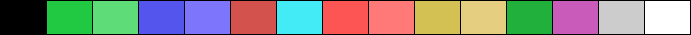
\includegraphics[scale=0.7]{images/TMS9918Apalette.png}

    \begin{itemize}
        \item VDP\_COLR\_TRNSP  (Transparent)   = \$00
        \item VDP\_COLR\_BLACK  (Black)         = \$01
        \item VDP\_COLR\_M\_GRN (Medium Green)  = \$02
        \item VDP\_COLR\_L\_GRN (Light Green)   = \$03
        \item VDP\_COLR\_D\_BLU (Dark Blue)     = \$04
        \item VDP\_COLR\_L\_BLU (Light Blue)    = \$05
        \item VDP\_COLR\_D\_RED (Dark Red)      = \$06
        \item VDP\_COLR\_CYAN   (Cyan)          = \$07
        \item VDP\_COLR\_M\_RED (Medium Red)    = \$08
        \item VDP\_COLR\_L\_RED (Light Red)     = \$09
        \item VDP\_COLR\_D\_YLW (Dark Yellow)   = \$0A
        \item VDP\_COLR\_L\_YLW (Light Yellow)  = \$0B
        \item VDP\_COLR\_D\_GRN (Dark Green)    = \$0C
        \item VDP\_COLR\_MGNTA  (Magenta)       = \$0D
        \item VDP\_COLR\_GREY   (Grey)          = \$0E
        \item VDP\_COLR\_WHITE  (White)         = \$0F
    \end{itemize}

    % ==========================================================================
    \subsection{VDP Screen resolutions}
    % ==========================================================================
    \label{sec:vdpscrmodes}


        % ==========================================================================
        \subsubsection{Mode 0: \textbf{Text Mode}}
        % ==========================================================================
        \begin{itemize}
            \item Screen is divided into 960 pattern positions each of which is
                capable of displaying a character. There are 40 characters in
                each row and 24 rows in total.
            \item Each character is 6 horizontal pixels by 8 vertical pixels.
            \item Each character can have 2 colours (Foreground and Background).
            \item Sprites cannot be used.
            \item Pattern Table:
            \begin{itemize}
                \item This table contains the character sets, for a maximum of
                    256 characters per set.
                \item Up to 7 different character sets can be held in the
                    \textbf{VRAM} at the same time. Each set MUST be located
                    starting at an \texttt{0x0800} boundary (i.e. 
                    \texttt{0x0000}, \texttt{0x1000}, \texttt{0x1800},
                    \texttt{0x2000}, \texttt{0x2800}, \texttt{0x3000} and
                    \texttt{0x3800}). Note that \texttt{0x0800} is not listed
                    because that address is used by the Name Table.
                \item Ideally, the patterns follow the ASCII table definitions
                    and order, so that the Name Table can be easily used to
                    display text by for example assigning the value \texttt{0x41}
                    to a byte in the Name Table to display the character
                    \textit{A}.
            \end{itemize}
            \item Name Table:
            \begin{itemize}
                \item Each entry in the table is 1 byte long and therefore can
                    specify one of 256 patterns (from \texttt{0x00} to
                    \texttt{0xFF}).
                \item Each entry represents a pattern position on the screen.
                    Position 0 is in the top left of the screen. Position 39 is
                    in the top right of the screen. The second row ranges from
                    40 to 79, and so on.
            \end{itemize}
        \end{itemize}

        % ==========================================================================
        \subsubsection{Mode 1: \textbf{Graphics I Mode}}
        % ==========================================================================
        \begin{itemize}
            \item Screen is divided into 768 blocks of 8x8 pixels each. There
                are 32 blocks in a row and 24 rows on the screen.
            \item Sprites can be used.
            \item Screen resolution is 256 by 192 pixels.
            \item Name Table:
            \begin{itemize}
                \item This table has 768 entries, one for each block on the screen.
                \item If the Pattern Table is loaded with with a full ASCII
                    character set, the entry of any ASCII value in the Name
                    Table will result in the corresponding character being
                    displayed on the screen.
            \end{itemize}
            \item Colour Table:
            \begin{itemize}
                \item This table has 32 entries, each entry defining 2 colours
                (Foreground and Background) out of 15 colours available, for a
                block of 8 characters. In other words, colours cannot be
                assigned independently to each character in the screen, but
                instead to groups of 8 consecutive characters.
            \end{itemize}
        \end{itemize}

        % ==========================================================================
        \subsubsection{Mode 2: \textbf{Graphics II Mode}}
        % ==========================================================================
        \begin{itemize}
            \item Screen is divided into 768 blocks of 8x8 pixels each. There
            are 32 blocks in a row and 24 rows on the screen.
            \item Sprites can be used.
            \item Screen resolution is 256 by 192 pixels.
            \item Name Table:
            \begin{itemize}
                \item This table is divided into three subtables of 256 each.
            \end{itemize}
            \item Colour Table:
            \begin{itemize}
                \item Each entry in the Colour Table is 8 bytes and each byte
                    defines the 2 colours (Foreground and Background) of each 
                    of the 8 rows of the character, from a total of 15 colours
                    plus transparent available.
            \end{itemize}
        \end{itemize}

        % ==========================================================================
        \subsubsection{Mode 3: \textbf{Multicolour Mode}}
        % ==========================================================================
        \begin{itemize}
            \item Screen is divided into 768 blocks of 2x2 squares. Each square
                is 4 pixels. There are 32 blocks in each row and 4 rows in each
                section. There are 6 sections, for a total of 24 rows on the
                screen.
            \item Blocks are arranged in columns with 4 blocks in each column.
            \item Columns are arranged in sections, with 32 columns in each
                section.
            \item There are a total of 6 sections on the screen.
            \item In summary:
            \begin{itemize}
                \item 32 columns * 6 sections = 192 columns
                \item 192 columns * 4 blocks = 768 blocks
            \end{itemize}
            \item No characters for text can be used.
            \item Sprites can be used.
            \item The Colour Table is not used. Instead, the colour of the boxes
            are defined in the Pattern Table.
            \item Pattern Table:
            \begin{itemize}
                \item Each entry in the table is 8 bytes, but only 2 bytes are
                        used to define the colours of the 4 boxes that make up
                        a character.
            \end{itemize}
        \end{itemize}

        % ==========================================================================
        \subsubsection{Mode 4: \textbf{Graphics II Mode Bitmapped}}
        % ==========================================================================
        \begin{itemize}
            \item Same as Mode 2, but screen is bitmapped for addressing every
                pixel individually.
            \item Pixels cannot have colours assigned individually. Instead
                colour is assigned by a byte, where each bit tells if the pixel
                is visible (bit=1) or not (bit=0). Therefore, pixels are grouped
                in groups of 8. For example, \texttt{0x4F} (0100 1111) will set
                pixels 0, 1, 2, 3 and 6 as visible, and pixels 4, 5, and 7 not
                visible. Pixels that are visible will have dark blue colour
                (\texttt{0x04}) over white background (\texttt{0x0F}).
        \end{itemize}

    % ==========================================================================
    \subsection{VDP Limitations}
    % ==========================================================================
    \label{subsec:vdp_limitations}

    The maximum resolutions are: 240x192 pixels in Text Mode, 256x192 pixels in
    Graphics Modes (I, II, II Bit-mapped), and 512x384 in Multicolour Mode.

    The maximum number of colours is 15 plus a transparent colour.

    In Graphics I Mode, each entry in the Colour Table defines the colour for
    a group of eight patterns. Hence, individual character colouring is not
    possible.

    In Graphics II Bit-mapped Mode, individual pixels can be addressed but
    individual colours cannot. Therefore it is not possible to assign different
    colours for each pixel.

    Bug?: After some tests, and confirmed with some information found on the
    Internet, reading continuously the Status Register can lead to miss the flag.
    This happens when the register is read and the VDP is about to set it,
    because as specified in the \textit{Video Display Processors Programmer's
    Guide}\cite{ti1}, \textit{the Status Register is reset after it's read}.
    Therefore, the subroutine implemented in dzOS for waiting for the VBLANK
    (\textit{BIOS\_VDP\_VBLANK\_WAIT}) that initially was reading the
    \textbf{VDP}'s Status Register and looping until the MSB changed to 1, has
    been changed to instead check for a change on the
    \hyperref[subsec:jiffy_counter]{Jiffy Counter}.

    % ==========================================================================
    \subsubsection{Sprites}
    % ==========================================================================

    A maximum of 32 sprites can be shown on the screen, of sizes either 8x8 or
    16x16 pixels. Though sprites can be magnified, thus showing as 16x16 or
    32x32 respectively.

    The location of a sprite is defined by the top left-hand corner of the
    sprite pattern.

    When more than one sprite is located at the same screen coordinate, the
    sprite on the higher priority plane will be shown.

    A maximum of 4 sprites can be displayed on the same horizontal line. If this
    rule is violated, the four highest priority sprites on the line are
    displayed normally, but the fifth and subsequent sprites are not displayed.

    The \textit{Coincidence Flag} (collision dectection) only indicates that
    any two sprites have overlapping bits, but it does not tell which sprites
    are. This must be calculated programatically.

    % ==========================================================================
    \subsection{Jiffy Counter}
    % ==========================================================================
    \label{subsec:jiffy_counter}

    A \textit{Jiffy} is the time between two ticks of the system timer interrupt.
    On the dastaZ80, this timer is generated by the TMS9918A (\textbf{VDP}) at
    roughly each 1/60th second.\\

    The counter is made of 3 bytes. Byte 1 is incremented in each \textbf{VDP}
    interrupt. Once it rolls over to zero (256 increments), the byte 2 is
    incremented. Once the byte 2 rolls over, the byte 3 is incremented. Once the
    three bytes together (24-bit) reach the value \texttt{0x4F1A00}, the three
    bytes are initialised to zero.

    \texttt{0x4F1A00} (5,184,000 in decimal) is the number of jiffies in 24
    hours: 24 hours x 60 minutes in an hour x 60 seconds in a minute x 60
    jiffies in a second.

    \textbf{IMPORTANT}: This counter MUST not be interpreted as an accurate
    clock, because when transferring data to the \textbf{VRAM} the OS disables
    the \hyperref[sec:nmi]{NMI}\footnote{It is also highly recommended that in
    your programs you also disable the \hyperref[sec:nmi]{NMI} when copying
    large amounts of data. Otherwise, the process will be interrupted 60 times
    per second, and therefore slow it down.}, and therefore the counter stops
    for a while.

    % ==========================================================================
    \subsection{OS Boot Sequence}
    % ==========================================================================
    After power on or after pressing the \textbf{RESET} button:

    \begin{itemize}
        \item \textbf{Bootstrap}
        \begin{itemize}
            \item Copy contents of the ROM into High RAM (\texttt{0x8000} - \texttt{0xFFFF}).
            \item Disable ROM chip and enable Low RAM (\texttt{0x0000} - \texttt{0x7FFF}).
            Therefore, all \textbf{MEMORY} is RAM from now on.
            \item Copy the copy of ROM inm High RAM to Low RAM. Bootstrap code is not copied.
            \item Transfer control to BIOS (\texttt{jp F\_BIOS\_SERIAL\_INIT}).
        \end{itemize}
        \item \textbf{Initialise SIO/2} (\texttt{F\_BIOS\_SERIAL\_INIT})
        \begin{itemize}
            \item Initialise SIO/2.
            \begin{itemize}
                \item Set Channel A as 115,000 bps, 8N1, Interrupt in all 
                received characters.
                \item Set Channel B as 115,000 bps, 8N1, Interrupt in all 
                received characters.
                \item Set Interrupt Vector to \texttt{0x60}.
            \end{itemize}
            \item Set CPU to Interrupt Mode 2.
            \item \texttt{jp F\_BIOS\_WBOOT}
        \end{itemize}
        \item \textbf{BIOS Boot} (\texttt{F\_BIOS\_WBOOT})
        \begin{itemize}
            \item Enable NMI (VDP) interrupts.
            \item Set NMI jump address to default value.
            \item Transfer control to Kernel (\texttt{jp F\_KRN\_START}).
        \end{itemize}
        \item \textbf{Kernel Boot} (\texttt{F\_KRN\_START})
        \begin{itemize}
            \item Display dzOS welcome message.
            \item Display dzOS release version.
            \item Display BIOS version.
            \item Display Kernel version.
            \item Display available \textbf{RAM}.
            \item Initialise \textbf{VDP}.
            \begin{itemize}
                \item Test write/read \textbf{VRAM}.
                \item Set \textbf{Low Resolution Display} as \textit{Graphics II
                Bit-mapped Mode}.
                \item Show dastaZ80 Logo in the \textbf{Low Resolution Display}.
            \end{itemize}
            \item Initialise \textbf{PSG}.
            \begin{itemize}
                \item Set Noise OFF, Audio OFF, I/O Port as Output.
                \item Make a beep.
            \end{itemize}
            \item Initialise \textbf{FDD}.
            \item Initialise \textbf{SD Card}.
            \begin{itemize}
                \item Detect \textbf{SD Card}.
                \item Display number of available Disk Image Files.
                \item Display disk unit and name of each Disk Image File.
            \end{itemize}
            \item Initialise \textbf{Real-Time Clock (RTC)}.
            \begin{itemize}
                \item Display current date and time.
                \item Display \textbf{RTC}'s battery status.
            \end{itemize}
            \item Initialise \hyperref[sec:ram_memmap]{SYSVARS}.
            \begin{itemize}
                \item Set show deleted files with \textit{cat} command as OFF.
                \item Set default File Type as 0 (USR = User defined).
                \item Set default loadsave address to \texttt{0x0000} (i.e. will
                save/load starting from \hyperref[subsec:memmap:ram]{Free RAM}
                (\texttt{0x4420})).
            \end{itemize}
            \item Set default \textbf{DISK} as 1 (i.e. first Disk Image File in
            the \textbf{SD card}).
            \item Transfer control to Command-line Interpreter (CLI) (\texttt{jp F\_CLI\_START}).
        \end{itemize}
        \item \textbf{CLI} (\texttt{F\_CLI\_START})
        \begin{itemize}
            \item Display CLI version.
            \item Clear command buffers
            \item Display prompt ($>$).
            \item Read command entered by user.
            \item Parse command.
            \item Execute corresponding subroutine.
            \item Loop back to Display prompt.
        \end{itemize}
    \end{itemize}

    % ==========================================================================
    \subsection{dzOS Programming Style}
    % ==========================================================================

    When writting dzOS and software for dzOS, the following style has been
    followed:

    \begin{itemize}
        \item All CPU registers are witten in uppercase (e.g. \textit{A},
        \textit{BC}, \textit{HL}, \textit{IX}, \textit{SP}).
        \item All CPU flags are witten in lowercase (e.g. \textit{z},
        \textit{nz}, \textit{c}, \textit{nc}, \textit{m}, \textit{p}).
        \item All assembly mnemonics are written in lowercase (e.g. 
        \textit{ld A,0}).
        \item Labels for subroutines that will be public (i.e. called via a
        Jumpblock) are written in uppercase.
        \item Labels are written in a line, with no mnemonics.
        \item Public subroutines contain comments specifying:
        \begin{itemize}
            \item Short description.
            \item Input CPU registers or variables (\hyperref[sec:ram_memmap]{SYSVARS}).
            \item Output CPU registers or variables (\hyperref[sec:ram_memmap]{SYSVARS}).
        \end{itemize}
        \item All hexadecimal values are written with a dollar sign as prefix.
        \item Tabulation (Tabs) are written as 4 spaces.
        \item Mnemonics start after 2 tabs (8 spaces).
        \item When possible, comments are written in column 41. Otherwise in
        next closest Tab.
        \item Source code is heavily commented. Mostly on each line.
        \item \textit{The Telemark Assembler} (TASM) specific:
        \begin{itemize}
            \item \textit{.BYTE} is used instead of \textit{.DB}
            \item \textit{.WORD} is used instead of \textit{.DW}
        \end{itemize}
    \end{itemize}

    % ==========================================================================
    \subsection{How a BASIC program is stored in RAM}
    % ==========================================================================

    When a user enters a program line (e.g. \texttt{10 PRINT "HELLO WORLD"}),
    BASIC must store it somewhere in \textbf{RAM} so that it can be retrieved
    later when for example the user wants to run, list or save the program.

    If all bytes would have to be stored, our example above would require 20
    bytes for the text code (including space between line number and PRINT),
    plus at least 2 bytes more for the line counter.

    The authors of MS BASIC cleverly decided that instead of storing the BASIC
    statements as ASCII characters, needing one byte per character, it would be
    enough to give each statement a unique identifier of one byte and instead
    store that byte. This unique identifier is commonly know as \textit{token}.

    For example, the \texttt{PRINT} statement has the token \texttt{0x9E}, so
    instead of needing 5 bytes to store each letter of the word \textit{PRINT},
    BASIC just needs 1 byte. It has saved 4 bytes. Imagine how much can save in
    a program with hundreds or even thousand of lines.

    So how it's a program stored in RAM, now that we know BASIC will use tokens
    for each reserved word instead of storing each character of the word?

    Lets take our previous example: \texttt{10 PRINT "HELLO WORLD"}

    Assuming the program is stored at address \texttt{0x80F9}, it will be stored
    as:

    \texttt{
    \resizebox{12cm}{!}{
        \begin{tabular}{l l l l l l l l l l l l l l l l l}
            80F9: & 00 & 0E & 81 & 0A & 00 & 9E & 20 & 22 & 48 & 45 & 4C & 4C & 4F & 20 & 57 & 4F\\
            810F: & 52 & 4C & 44 & 22 & 00 & 00 & 00\\
        \end{tabular}
    }}

    where:

    \begin{itemize}
        \item \texttt{00}: flag indicates start of program.
        \item \texttt{0E 81}: address to the next line in memory. In this
        example equals to end of program as there are no more lines.
        \item \texttt{0A 00}: line 10 in little-endian.
        \item \texttt{9E}: token for PRINT.
        \item \texttt{20}: space character.
        \item \texttt{22}: double quote (") character.
        \item \texttt{48 45 4C 4C 4F}: characters for HELLO.
        \item \texttt{20}: space character.
        \item \texttt{57 4F 52 4C 44}: characters for WORLD.
        \item \texttt{22}: double quote (") character.
        \item \texttt{00}: flag indicates end of line.
        \item \texttt{00 00}: flag indicates end of program.
    \end{itemize}

    Now it's easy to understand why some programs published in books and
    magazines skip some of the blank spaces, and write \texttt{FOR I=0 TO 10}
    instead as \texttt{FORI=0TO10}. It saves 3 bytes in memory by not having to
    store the space characters \texttt{0x20}. It also increases a bit the
    running speed, as the BASIC interpreter doesn't have to parse and interpret
    each of the spaces.

    % ==========================================================================
    \subsection{How a BASIC program is stored in DISK}
    % ==========================================================================

    \begin{itemize}
        \item 2 bytes: Address of PROGND (End of program). Start of variables
            area. This is where the variables are stored.
        \item 2 bytes: Address of VAREND (End of variables). Start of arrays
            area. This is where the arrays are stored.
        \item 2 bytes: Address of ARREND (End of arrays). This contains the
            address of the byte after last array.
        \item 2 bytes: Address of NXTDAT (Next DATA item). This contains the
            address of the next item of DATA to be READ.
        \item 2 bytes: Address of FNRGNM (FN argument name). This contains the
            name of the argument for the current FN function.
        \item 4 bytes: Address of FNARG (FN function argument). This is the
            floating point value of the current FN function's argument.
        \item 4 bytes: Address of FPREG (Floating point register). This is a
            floating point number for the current value.
        \item 1 byte: Address of SGNRES (Sign of result). This contains the sign
            of the result for multiplication.
        \item 13 bytes: Address of PBUFF (Number print buffer). When a floating
            point number has to be converted into ASCII for PRINT or STR\$ the
            ASCII number is built up in this buffer.
        \item 3 bytes: Address of NULVAL (Multiply value). This contains the
            24-bit multiplier.
        \item n bytes: tokenised BASIC program.
    \end{itemize}


    \pagebreak
    % ==========================================================================
\section{Glossary}
% ==========================================================================

\begin{itemize}
    \item \textbf{Block Allocation Table (BAT)}: is a data structure used to
        track disk blocks on a \textbf{DISK}. The Table is used as index of
        files, and each entry in the Table constains details about each file
        (filename, attributes, size, etc.) and details on how the OS can access
        the data (e.g. in which Sector the file is stored). Technically, the BAT
        is not allocating Blocks but Sectors, so it should have been named
        Sector Allocation Table instead.
    \item \textbf{BIOS}: The Basic Input/Output System is the firmware used to
        provide hardware related subroutines to the operating system. It is
        stored in an EEPROM that cannot be modified unless extracting the chip,
        but during the boot sequence the entire OS (BIOS, Kernel and CLI) are
        copied into RAM.
    \item \textbf{CLI}: The Command-Line Interface is the part of the operating
        systems that is in charge of reading and interpreting input entered by
        the user and outputting information back to the user.
    \item \textbf{Composite video}: Composite video (also knows by CVBS) is an
        analog video format that combines, on one wire, the video information
        required to recreate a colour picture, line and frame synchronisation
        pulses. A yellow RCA connector is typically used for this type of signal.
    \item \textbf{CPU}: A Central Processing Unit is the chip that executes
        instructions and I/O operations. In the case of the dastaZ80, the CPU is
        a Zilog Z80 running at 7.3728 Mhz.
    \item \textbf{Disk Image file}: A disk image file contains a snapshot of a
        bit-by-bit copy of a storage device's structure. In the case of dastaZ80,
        this structure is defined by the characteristics of the DZFS (dastaZ80
        File System). Each image file can be understood as a separate hard disk
        connected to the computer, but in the form of a file instead of being a
        physical hard disk drive.
    \item \textbf{DZFS}: dastaZ80 File System is a file system of my own design,
        for storage devices, aimed at simplicity. It allows Disk Image files of
        a maximum of 33 MB for a maximum of 1024 files in each image. Each file
        can be a maximum of 32 KB in size.
    \item \textbf{EEPROM}: Electrically Erasable Programmable Read-Only Memory
        is a type of non-volatile memory that can be erased and re-programmed.
    \item \textbf{File System}: A file system manages access to the data and the
        metadata of the files, and the available space of the device, dividing
        the storage area into units of storage and keeping a map of every
        storage unit of the device.
    \item \textbf{General-Purpose Input/Output (GPIO)}: is a set of pins which
        carries \textbf{CPU} (among others) signals, and allows external devices
        to be plugged into the GPIO connector an be managed by the computer.
        Typical devices connected to a GPIO are; modems, RAM expansions,
        Real-Time Clocks (RTC), hard drives.
    \item \textbf{Kernel}: The Kernel is a layer of the operating system that
        it is in between the software and the BIOS. Thus the Kernel is agnostic
        to the hardware, and is only responsible for calling the needed
        subroutines.
    \item \textbf{Logical Block Addressing (LBA)}: is a scheme for specifying
        the location of blocks of data stored on computer storage devices. In
        DZOS, it is based in blocks of sectors, where each block is 64 sectors
        a each sector is 512 bytes.
    \item \textbf{LED}: A Light-Emitting Diode is a semiconductor device that
        emits light when current flows through it. It is commonly used in
        computers, as light indicator, due to their high durability and low
        power consumption.
        \item \textbf{NTSC}: National Television System Committee, is the
        standard for analog television used mainly in USA, Japan and some parts
        of South America.
    \item \textbf{PAL}: Phase Alternating Line (PAL) is the standard for analog
        television used mainly in European countries, some African countries,
        some Asian countries, and some Soth American countries.
    \item \textbf{RAM}: Read-Access Memory is a type of volatile memory, that is
        generally used for storing temporary data, like for example programs
        loaded from disk or input entered by the user.
    \item \textbf{RCA connector}: Is a type of electrical connector commonly
        used to carry audio and video signals. It is also called
        \textit{phono connector}. The standard is to have yellow connector for
        video, and white and red for audio.
    \item \textbf{ROM}: Read-Only Memory is a type of non-volatile memory that 
        cannot be electronically modified after the manufacture process.
    \item \textbf{Sector}: A virtual group of 512 bytes stored in a
        \textbf{DISK}. 
    \item \textbf{Superblock}: The first 512 bytes on a \textbf{DISK} contain
        fundamental information about the \textbf{DISK} geometry, and is used by
        the OS to know how to access every other information on the
        \textbf{DISK}. On IBM PC-compatibles, this is known as the
        \textit{Master Boot Record} (MBR). I decided to call it
        \textit{Superblock}, as it is an orphan Sector that doesn't belong to
        any Block and it's physically store above any other Block.
    \item \textbf{TTL}: Transistor-Transistor Logic is a family of digital
        integrated circuits. The important thing to know for the usage of the
        dastaZ80 is that standard TTL circuits operate with a 5 Volt power
        supply.
    \item \textbf{VGA}: The Video Graphics Array is a video display controller
        that became the standard for video output for computers around 1990s,
        and remained until the introduction of other standards around 2000s.
\end{itemize}
    \pagebreak

    % ==========================================================================
    % Bibliography
    % ==========================================================================
    \pagebreak
    \bibliographystyle{unsrt}
    \bibliography{../dastaZ80}
\end{document}
